\chapter{On-Body Placement}
\label{chapter:onbody}
    %\vspace*{\beforechapskip}%
    %\smash{\rule{2.6pt}{25mm}}
 %\chapterprecis{
\begin{flushright} 
\textit{"All models are wrong, but some are useful."
-George E. P. Box}
\end{flushright} 
%}
\begingroup %\vspace*{\beforechapskip}% %\smash{\rule{2.6pt}{25mm}}
\textit{Coarse variations related to the on-body placement of a device
  have a high impact on the reliability and effectiveness of context
  recognition systems. This chapter explores how changes in on-body
  placement impact sensing modalities commonly used in pervasive
  computing. We discuss general considerations and give some advice on
  how to make activity sensing more robust to placement changes.  We
  then present several methods to derive the coarse device
  placement solely based on rotation and acceleration signals. 
  The methods work regardless of device orientation.  We
  present an elaborate evaluation of these methods on already
  published, large scale data sets with diverse activities from
  bicycle repair to house work.  We reach a recognition rate of 80\%
  over 4 min. of unconstrained motion data for the worst scenario and
  up to 90\% over a 2 min. interval for the best scenario.}\\\\ 
K.~Kunze and P.~Lukowicz.  \newblock Using acceleration signatures
from everyday activities for on-body device location.  \newblock {\em
  11th IEEE International Symposium on Wearable Computers}, Sep 2007.
\\K.~Kunze, P.~Lukowicz, H.~Junker, and G.~Troester.  \newblock Where
am i: Recognizing on-body positions of wearable sensors.  \newblock
{\em LOCA'04: International Workshop on Location and Context Awareness
}, Jan 2005.

\vskip\onelineskip
\begin{adjustwidth}{}{-\chapindent}%
\hrulefill   
\end{adjustwidth}\endgroup
\vskip\onelineskip
\vskip\onelineskip 
After discussing general environmental placement issues, we focus on
lifting another constraint for the users: Having to place sensing devices on
well-defined positions on the body. 
\begin{figure}[t]
    \begin{center}
    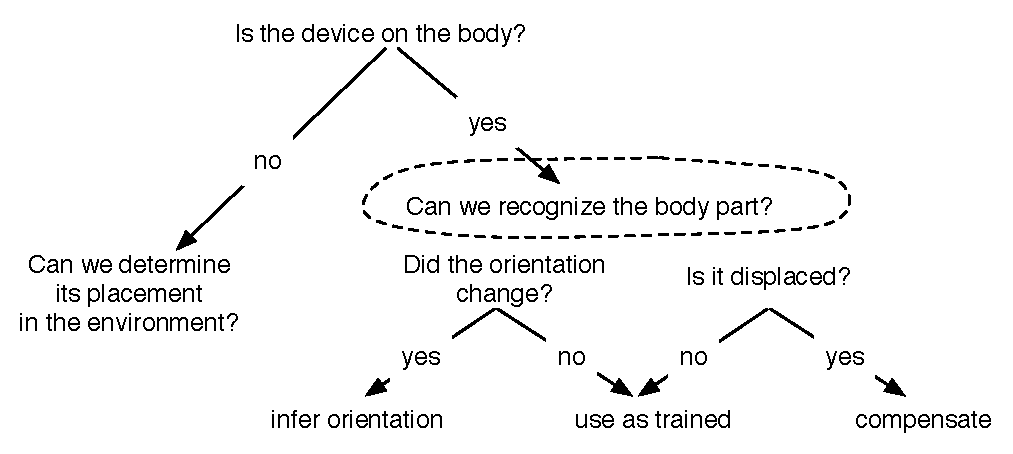
\includegraphics[height=2in]{OnbodyOverview}
	\end{center}
\caption[Focus of the On-body Placement Chapter]{Thesis overview with the central question for this chapter
  highlighted.} \label{fig:onbodyoverview} \end{figure} 
Specifically, this chapter deals with coarse variations related to the body part, on 
which the device is carried (see in Figure~\ref{fig:onbodyoverview}).

A well-established approach to context and activity
recognition is the use of motion sensors (predominantly
accelerometers) attached to different parts of the user's body.
Various types of activities ranging from simple modes of locomotion
analysis to complex assembly tasks have been successfully recognized
using such sensors~\cite{seon2001recognition,bao2004activity,lukowicz2004recognizing} .  
Most research in this area, however, relies on sensors being placed at specific
locations on the body. Typically, these include the wrists, the arms,
legs, hips, the chest and even the head. Once a subset of placements
is chosen, the system is trained on this specific subset and
will not function properly if the sensors are placed at different
locations.  This implies that the user either has to explicitly "put
on" the sensors each time he dresses up or the sensors have to be
permanently integrated into the individual pieces of clothing or
devices he usually carries, e.g. a mobile phone. If devices are used,
the user is required to carry them always at the same body location, e.g. the key chain needs to be
always placed in the right trouser pocket. 

We consider this to be a very critical issue. Experience shows that
people usually have several accessories with them and vary their
on-body placement depending on the circumstance~\cite{Ichikawa:2005p6295}. In a
typical scenario the user might carry a key-chain in his trousers
pocket giving us the leg information, a watch on the wrist, a mobile
phone in a holster on the hip and a smart card in the wallet in a jacket
pocket. A flexible context recognition system could then 
determine the on-body location of the devices to use them for an inference task.

Location information in itself is an interesting part of
context. As an example, knowing if glasses are worn or if they are in
a pocket can be an important clue to the user's activity.

The work described in this chapter is a major step in our effort to
facilitate the adaption of context recognition
with one focus: learning the device placement on the body. We
illustrate on-body placement issues on sensor modalities common in
activity sensing. Then, we explore how to classify different body
placements. To assess the feasibility, we start with a very
narrowly defined activity, namely "walking". We demonstrate how to
detect "walking" in a device placement independent way and then
leverage this to detect the device placement. In the following, we can abstract a
more general model, no longer constraint to 'walking'. The model works for a broad range of common human
activities tested in a large scale experimental evaluation.

% We then demonstrate how the
%information that the user is walking can be leveraged to determine
%device location.



\section{Impacts of the Body Part Placement}
\begin{figure}[!t]
\centering
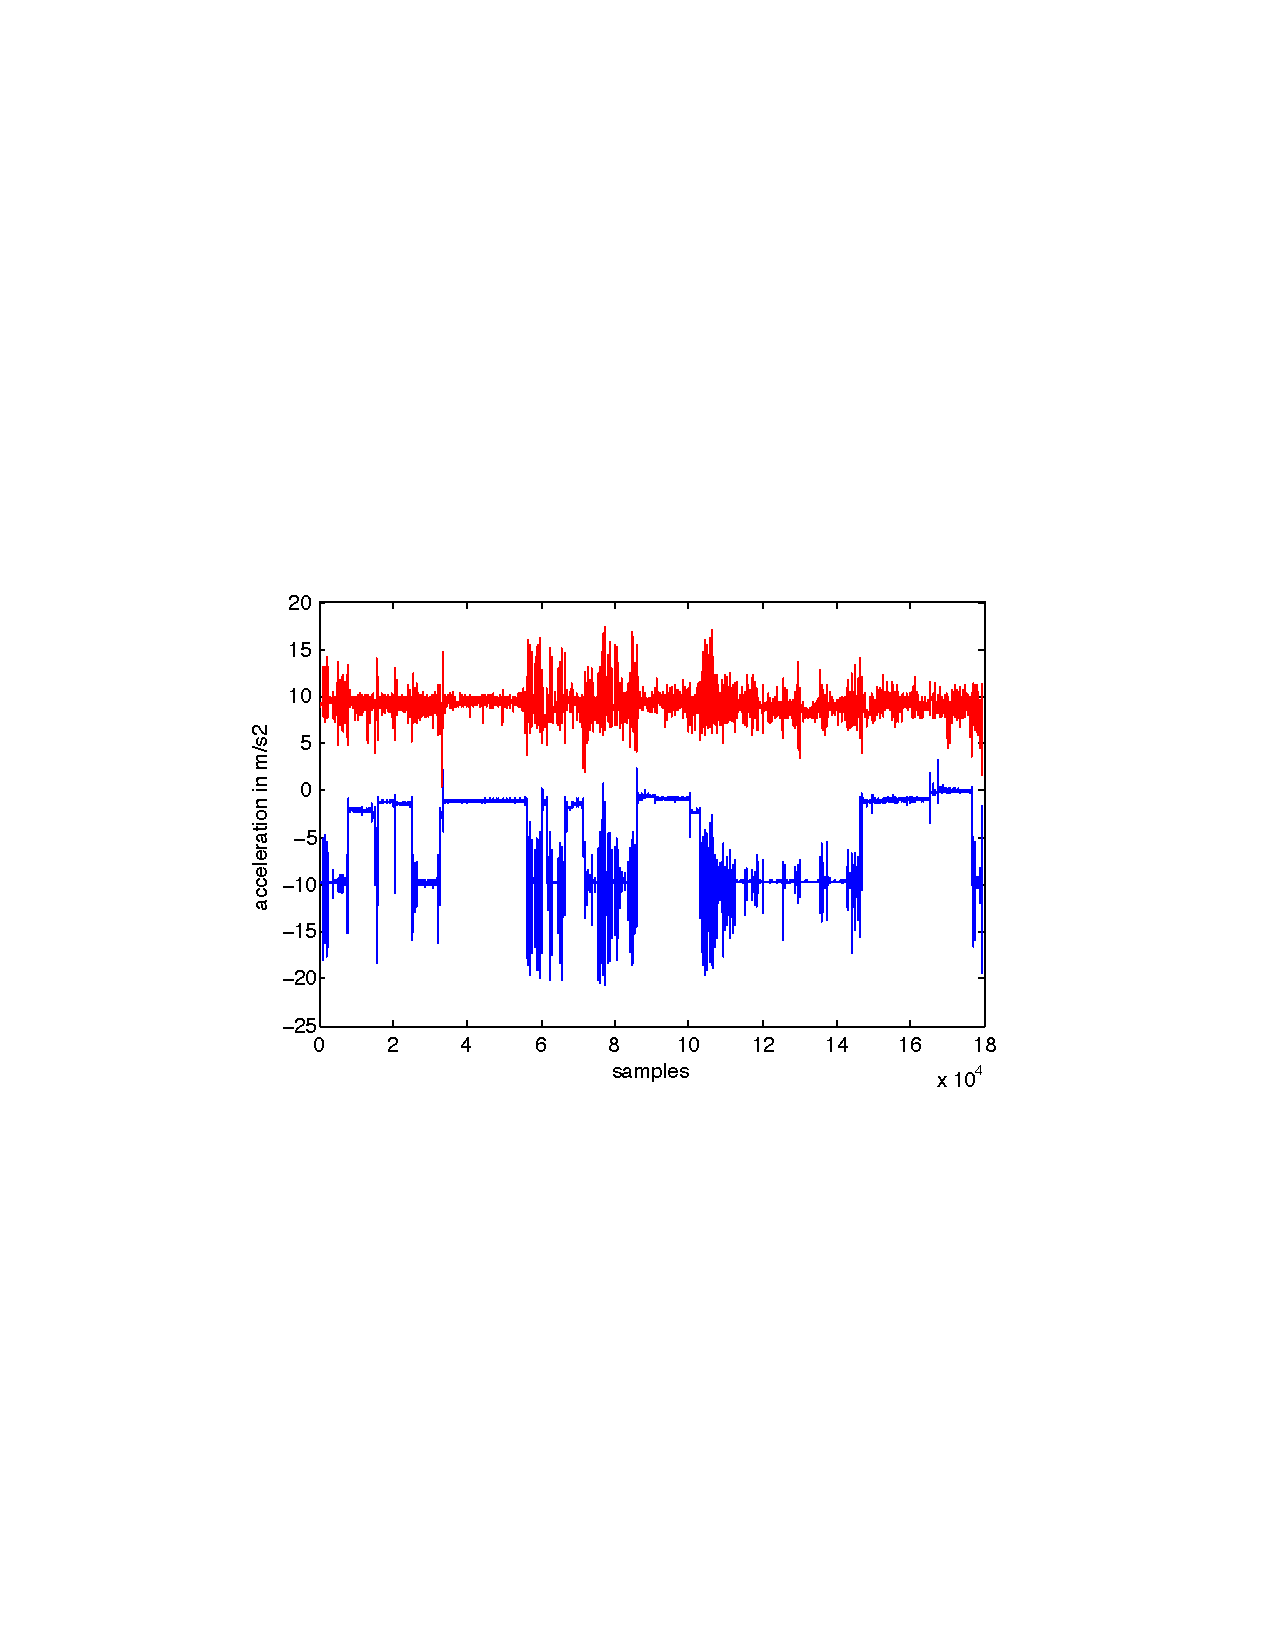
\includegraphics[width=2.9in]{acceleration}
\caption[Body placement impacts on an accelerometer]{Body placement impact on an accelerometer signal; shown here is the 
horizontal axis of a sensor attached to the wrist (top), 
versus a sensor placed in the right trouser pocket (bottom). 
One can clearly see the sitting sections and the shifts in the gravity vector 
due to orientation changes of the sensor. The plot is from the House Work dataset.}
\label{fig:obacceleration}
\end{figure}
\begin{figure}[!t]
\centering
\includegraphics[width=5in]{3onbodyWalking}
\caption[Acceleration: Walking versus not walking]{Accelerometer Signal, vertical axis for walking and not walking.}
\label{fig:walking}
\end{figure}
\begin{figure}[t]
    \begin{center}
    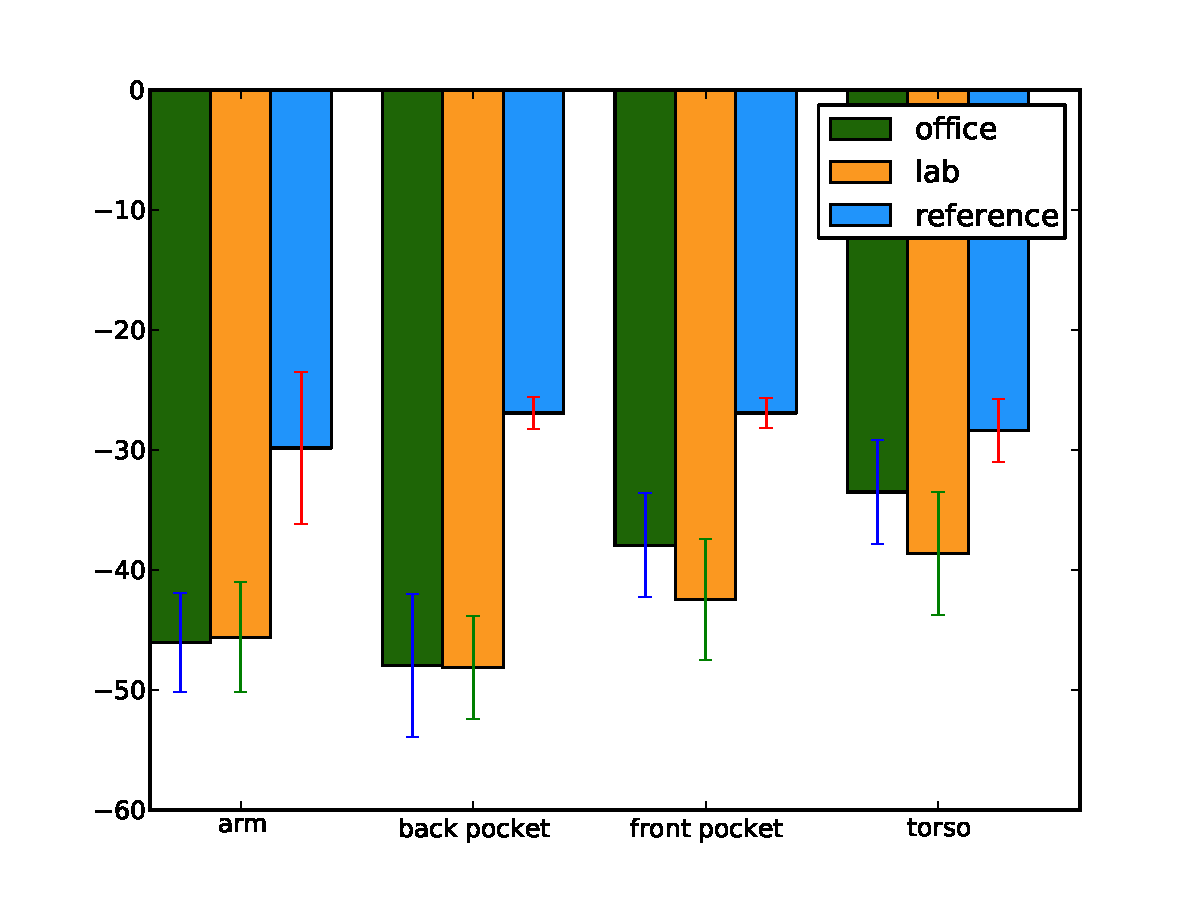
\includegraphics[height=2.9in]{sigstrength.pdf}
	\end{center}
\caption[WIFI signal strength dependent on body placement]{WIFI signal strength depending on on-body location of the
  mobile phone. The phone is put on a specific body location for 5
  minutes stationary in several rooms: in one office, laboratory, and on
  the corridor between the two as reference. The experiment is
  repeated 15 times. We show the mean average signal strength in the
  plot.}  \label{fig:sigstrength}
\end{figure}
Obviously, signals from motion related sensors such as accelerometers,
gyroscopes and magnetic field sensors are significantly
influenced by the body part, on which the device is placed.  

Compared
to sound or radio signals, motion signals are more closely linked to the on-body
placement and not dependent on the absorption spectra of clothing or similar. The
influence of the body placement on motion signals is twofold. First,
some activities are associated with specific body parts. Sensors in
other locations contain no or little related information. For example,
activities related to subtle arm motions (e.g. screw driving, or
washing hands) produce nearly no motion related signals in torso- or
leg-mounted sensors, unless the motion is strong enough that the torso
vibrates in sync with the hand motions. "Sitting down" and "standing
up" also have a characteristic signature for an accelerometer on the
upper leg (e.g. in the trouser pocket see Figure~\ref{fig:obacceleration}). Yet, they are nearly
impossible to distinguish from a belt mounted accelerometer. Second,
even for activities which are not strictly body part specific the
motion sensor signals vary significantly between different body
locations (see placement dependent signals in Figure~\ref{fig:walking} while the user is walking).
The same holds for gyroscopes. Figure~\ref{fig:drinking} shows gyroscope signals recorded form the lower arm and the head. 
In contrast to the gyroscope however,  an accelerometer signal contains always static and dynamic acceleration.
The static part is due to gravity, the dynamic part due to the user's motion. Both of them are not easily separable (see Figure~\ref{fig:obacceleration}).

\begin{figure}[t]
    \begin{center}
    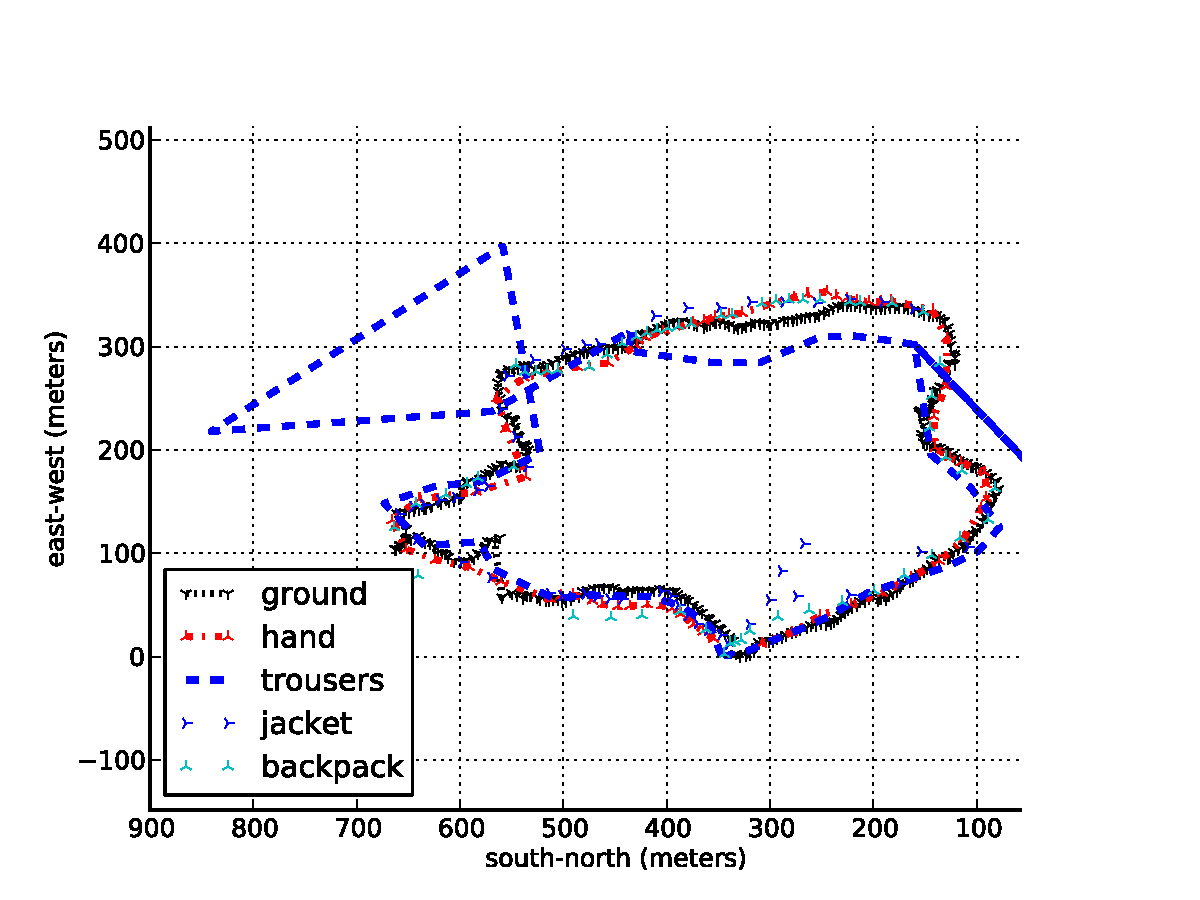
\includegraphics[height=2.9in]{city2.pdf}
	\end{center}
\caption[Body placement impact on GPS]{GPS traces using the same route
recorded with the device at different on body placements.
Three different mobile phones were placed in
each of the following locations: hand, front pocket of trousers, inner
pocket of the jacket, inside a backpack. The experimental study
contains over 50 km of traces in different environments. The error for the mobile phone placed in the
trouser pocket are by far the highest.  The analysis shows that
depending on the location on which the device is being carried, the
average error can increase by as much as 50\%. }  
\label{fig:gps} 
\end{figure}

Motion sensors and microphones, however, are not the only sensing modalities
influenced by the on-body placement. As shown in
Figure~\ref{fig:sigstrength}, WIFI signal strength, often used for
indoor positioning, is also dependent on the on-body placement of the sensor. This is
due to the large damping effect of the human body.  A similar effect
can be observed for GPS signals. This is illustrated in
Figure~\ref{fig:gps}. Interestingly, the GPS location fix is worst when the device is placed in the pocket,
a very common on-body placement for smart phones.

As already discussed in Chapter~\ref{chapter:OnOff}, an obvious
example of another sensing modality influenced by the on-body location is
sound. Regarding sound, the signal impacts are related less
to body damping and more to the absorption spectra of their surrounding, e.g. clothing.
The absorption spectra for some often used types of clothing
are shown in Figure~\ref{fig:soundplacement}. We already discussed how this fact can be used
to recognize symbolic locations, including some body part placements, 
see Chapter~\ref{chapter:OnOff} for details.


As shown above, common sensors used in context
recognition are influenced by their placement on the body. We
summarize our findings in the following:
\begin{itemize}
	\item Radio communication from devices carried on the body is
          influenced by body dampening.  It depends on the frequencies
          used and body part placement. Our examples, WIFI and
          gps, show that the influences can be statistically
          significant.
        \item Sound might also be influenced by body
          dampening. However, the most dominant impact on sound is the
          absorption spectrum of the clothing and compartment in which
          the device is carried.
        \item The signals from motion sensors are highly specific to
          the on-body placement, even if they originate from movements
          of the user's whole body.
\end{itemize}


\section{Related Work}

Most research work focuses on aggregating sensor data to become device
placement independent. Van Laerhoven et. al. present simple switch
sensors and show that they are less body placement dependent with
similar recognition rates for some activity recognition
tasks compared to accelerometers~\cite{vanLaerhoven:2004p1442}.  
Lester and Krause describe how to use sensor fusion methods 
to achieve device placement independent
recognition~\cite{Lester:2006p856,Krause:2003p1536}. The activity
recognition classes they can detect, however, are still rudimentary,
e.g. modes of locomotion. Kern et. al.  follow a similar approach
using a multitude of different sensors ~\cite{kern2003multi}.  Lester
et. al. present how to detect if two devices are carried by the same
person or different people~\cite{Lester:2004p738} in a device
placement independent way.  Other interesting complimentary work comes
from Blanke et. al. They fix the body placement (in the pocket) and
infer the symbolic location of the
wearer~\cite{Blanke:2008p6128}. Laerhoven et. al. train recognition
models adaptive to placement issues, yet they need direct user
feedback for training~\cite{laerhoven2000what}.

The work closest to the one presented in this chapter is by
Thiemjarus. She describes how to detect device orientation before
applying activity recognition~\cite{Thiemjarus:2010p10602}.  This is
complementary to the work we present here. Work related to device
orientation will be discussed in greater detail in
Chapter~\ref{Chapter:Orientation}.

\section{General Considerations}
There are two basic strategies to deal with different on-body
placements for activity recognition. The first is quite simple: one
can aggregate the sensor signals into features that are placement
independent, for example using the norm vector from a three axis
accelerometer. However, aggregation can only help 
little regarding such coarse variations as on-body placement, e.g. an
aggregated accelerometer signal from the arm will still differ to a large degree
from a signal recorded from the foot. The second strategy is to detect
the actual device placement or present heuristics to deal with changes
in placement.

\begin{figure}[!t]
\centering
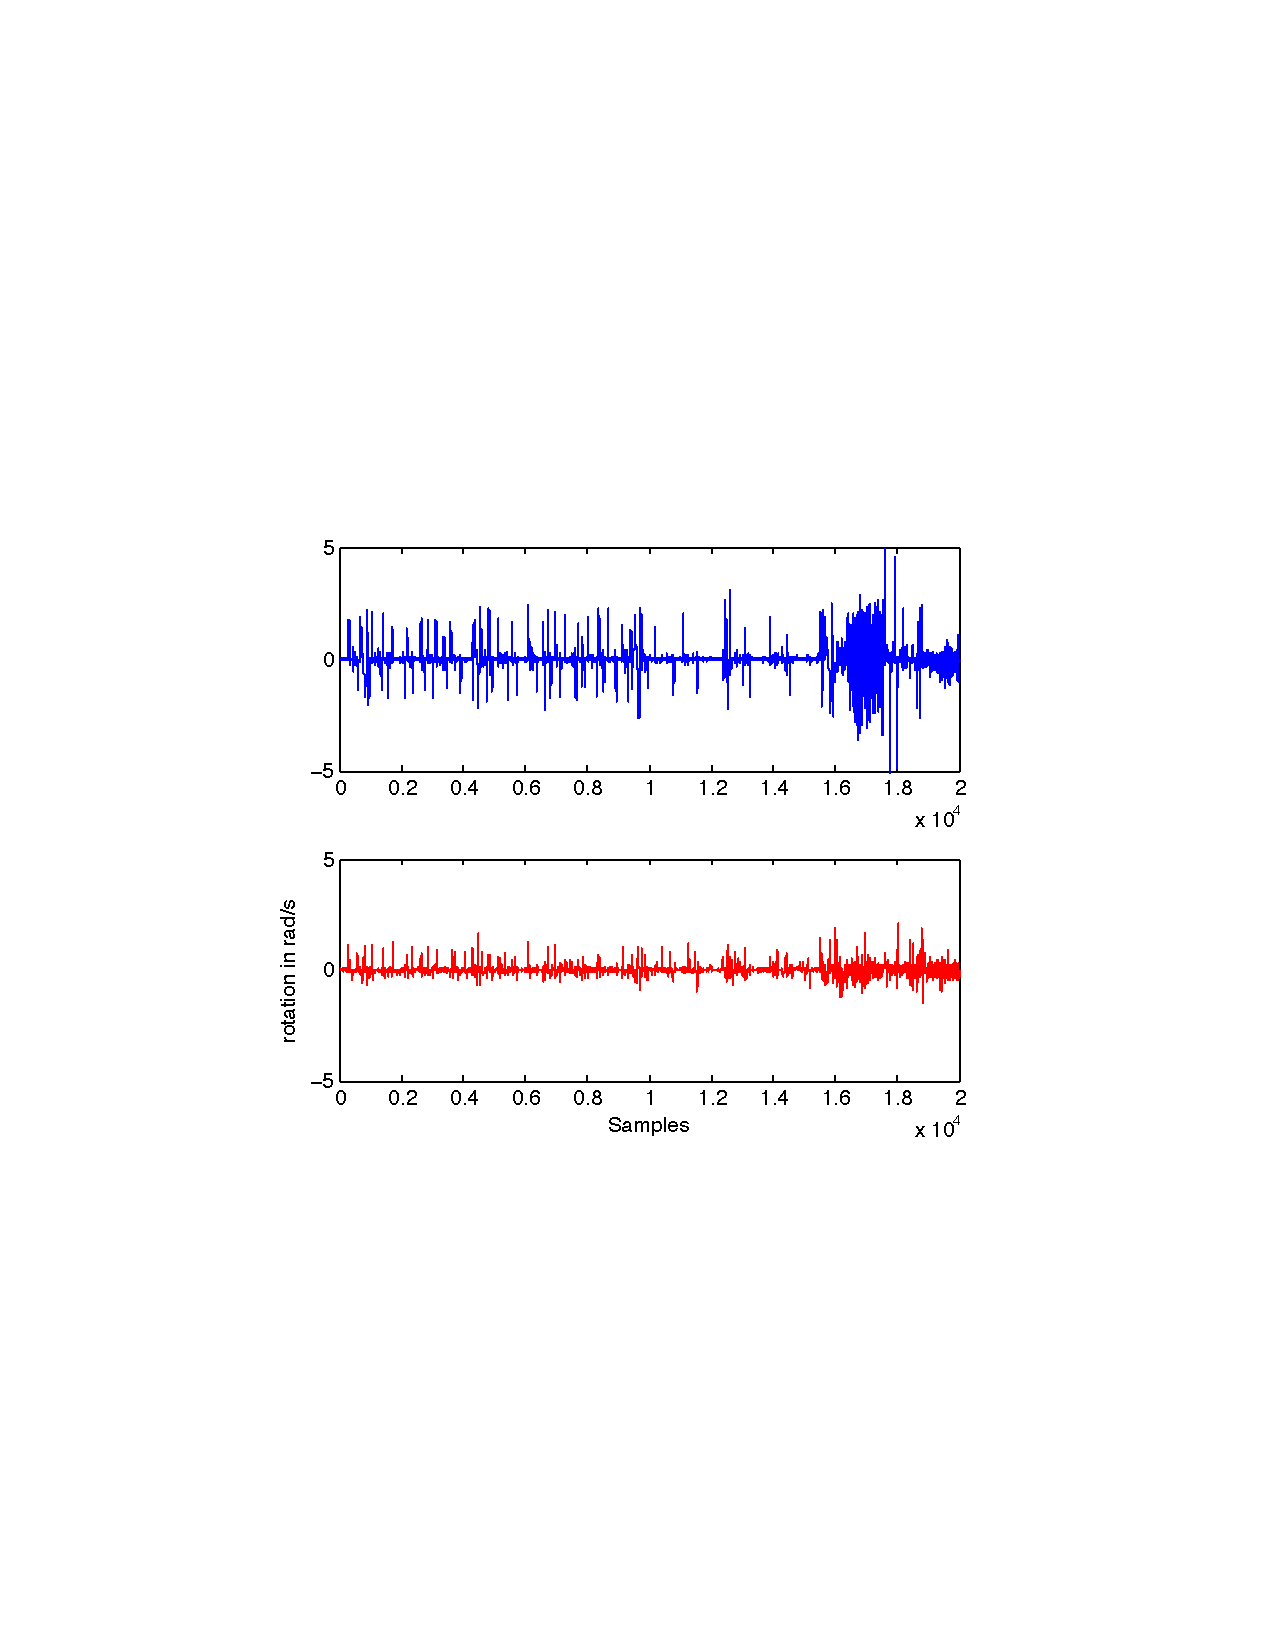
\includegraphics[width=2.9in]{drinking}
\caption[Body placement impact on a gyroscope]{gyroscope signal example, horizontal axis for drinking gestures,
  on the top a sensor attached to the lower arm, on the bottom a
  sensor attached to the left side of the head.  Although the movement
  is closely related, as drinking involves also tilting the head, the
  signals are clearly distinguishable.}
\label{fig:drinking}
\end{figure}

Our approach is based on the obvious observation that different parts
of the body tend to move in different ways. As an example, hand
motions contain many more high frequency components and larger
amplitudes than hip or head motions.  To illustrate this,
Figure~\ref{fig:drinking} depicts the gyroscope signal for the drinking
gesture for two distinct body parts, the lower arm in the top graph
and the head in the bottom graph. Clearly, the lower arm shows higher angular 
velocities in average.  Taking into account physiological
constraints, certain types of motions are not permissible at
all for some parts of the body e.g. you can not turn your leg around
the vertical axis over the knee or tilt your head more than 90 degrees.
Additionally, some parts tend to be motionless for longer periods of time than
the others. Thus, in theory, a statistical analysis of the motion
patterns over a sufficient period of time should be able to provide
information about the location of a sensor on the body.

When implementing this idea in practice, however, one has to deal with
a number of issues. For one, the value of such a statistical analysis
depends on the user activity during the analysis window. Little
information will be gained, for example, if the user is sleeping the
whole time. Furthermore, the signal of a motion sensor placed on a
given body part is a superposition of the motion of this body part and
the motion of the body as a whole. Thus, while it is not possible to
tilt the head more than 90 degrees, such a tilt will be registered
when the user lies down. Finally, many of the motion characteristics
that can be used to distinguish between body parts involve absolute
orientation, which is hard to detect, in particular if the orientation
of the sensor is unknown.


\section{On-Body Placement Recognition} 

\begin{figure}[!t]
\centering
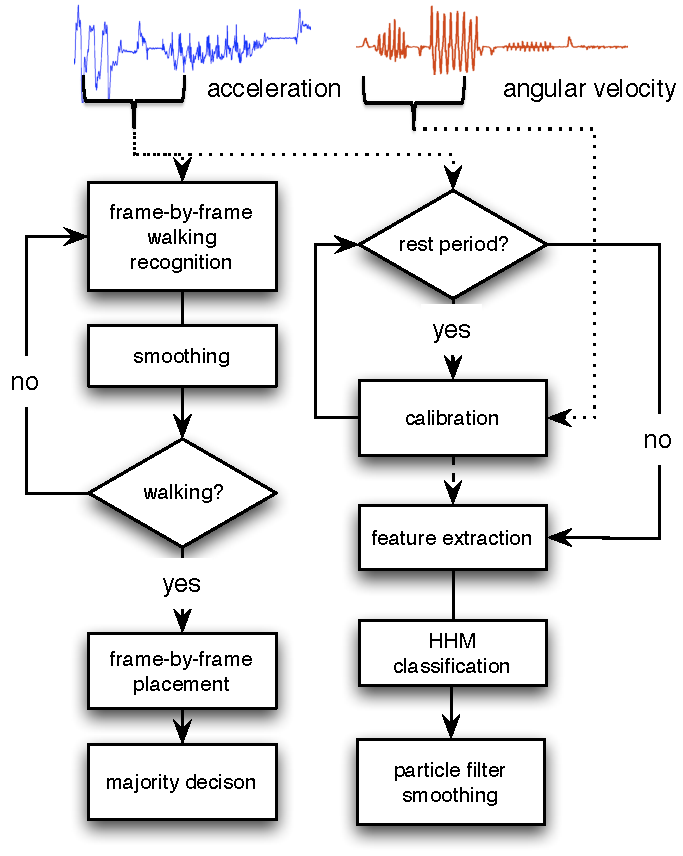
\includegraphics[width=3.5in]{onbody-overview}
\caption[On-body placement detection method]{Method overview, on the left the walking recognition only
  approach, on the right the HMMs with particle
  filtering.}  \label{fig:onbody-overview} \end{figure}

Although there are significant motion differences between body parts, human movement patterns are often 
irregular and sporadic. Therefore, limiting the recognition first to specific moments could be helpful.
We leverage the findings discussed in the considerations section and introduce in
this section two methods to detect the on-body placement of a motion
sensor shown in Figure~\ref{fig:onbody-overview}.  First, we explore
the "Walking Segment Method", the left part of
Figure~\ref{fig:onbody-overview}, based on accelerometer data alone.
It constrains the body part placement recognition to the time the user
is walking.  Afterwards we deal with a
basic time-series approach using Hidden Markov Models on both
accelerometer and gyroscope data. The latter approach works on unconstrained movement data
with the cost of increased complexity.

\subsection{Walking Segments Method}

A major issue to on-body detection are the the
wide range of irregular, sporadic movements a user might do. The
walking segments method tackles this problem in two ways:
\begin{enumerate}
\item The analysis is constrained to the time during which the user is
  walking.  This is motivated by two considerations.  First, walking
  is a common activity that occurs fairly often in most
  settings. Thus, being able to detect the position of devices during
  walking phases should provide us with a sufficiently accurate
  overall picture of where the devices are located. Moreover, once
  the location has been determined during a walking phase, this
  knowledge can be used to detect possible changes in placement.
  Walking has also a very distinct motion signature, that 
  can be recognized in an on-body placement indifferent way~\cite{sekine2000,seon2001recognition}.
\item We base our analysis on the norm of the acceleration vector
  which is independent of the sensor orientation.  
\end{enumerate} 

As you can see from Figure~\ref{fig:walking}, walking provides us with
a repetitive pattern, still maintaining distinct properties even for
different body locations. Thus, a simple sliding window, frame-by-frame
recognition approach with majority decision smoothing window should work for
this problem.


\begin{table}
\caption{Features used for the Walking Segments Method}
\begin{tabular}{p{5cm} p{8cm}}
\toprule 
RMS& $\sqrt{\frac{1}{N}*\sum_i{x_i^2}}$, where $N$ is the number of
samples a sliding window contains, and $x_i$ the i'th sample of the
window.\\ \midrule

75\%Percentile& Given a signal s(t) the 75\%percentile,
also known as the third quartile, is the value that is greater than
75\% percent of the values of s(t) .\\
\midrule

InterQuartileRange& The inter-quartile range is defined as the
difference between the 75th percentile and the 25th
percentile.\\ \midrule

Frequency Range Power& Computes the power of the
discrete FFT components for a given frequency band. \\ 
\midrule

Frequency Entropy& The frequency entropy is calculated according to
the following formula: $H_{freq}=-\sum{p(X_i)*log_2(p(X_i))}$, where
$X_i$ are the frequency components of the windowed time-domain signal
for a given frequency band and $p(X_i)$ the probability of $X$.  Thus,
the frequency entropy is the normalized information entropy of the
discrete FFT component magnitudes of the windowed time-domain- signal
and is a measure of the distribution of the frequency components in
the frequency band (see~\cite{bao2003physical}).\\\midrule
Sums Power Wave Det. Coefficient&  describes the power of the detail signals
at given levels that are   derived from the discrete wavelet transformation of the windowed
time-domain signal.  This feature has
  successfully been used to classify walking
  patterns with  acceleration sensors(\cite{sekine2000}). \\

\bottomrule
\end{tabular}     
\label{table:featuresWalking}
\end{table}

\subsubsection{Walking Recognition}
Basic physical considerations confirmed by initial tests, using over
40 features and information gain as selection criteria, lead us
to use the features given in Table~\ref{table:featuresWalking}
which we compute in one second sliding window (overlapping 0.5 sec.) over the acceleration signal from the device.
The "walking" recognition is trained in a location independent manner
by combining the data from multiple on-body locations into a single training set.  
Several standard machine learning algorithms are tested (e.g. C4.5, KNN). In the next phase, data
collected during walking is used to train the placement recognition.

\subsubsection{Placement Recognition}
\label{rec}

\begin{figure}[!t]
\centering
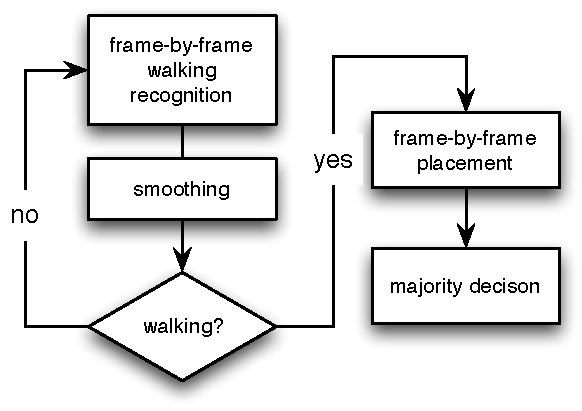
\includegraphics[width=3.5in]{walking-segment}
\caption{Overview of the walking segmentation method}  
\label{fig:walking-segment} 
\end{figure}
The recognition of the sensor placement is performed separately for each sensor using the
system trained according to the method described above. It consists of
the following steps, as also depicted in
Fig.~\ref{fig:walking-segment}:
\begin{enumerate}
\item{\em Frame by Frame Walking Recognition}
In this phase the features are computed in a sliding  window of length
1s as described above and each window is classified as walking or non
walking. The window length has been selected such that in a typical case
it contains at least one step.
\item{\em Walking Recognition Smoothing} Using another sliding window
  of length 10 sec moving by 5 sec the results of the frame by frame
  walking classification are then smoothed. The smoothing retains only
  those windows, where more then 70\% of the frames are classified as
  walking. This ensures that the subsequent location classification is
  based only on 'clean' walking segments.
\item{\em Walking Segment Localization} The smoothed frame-by-frame
  recognition results are then used to localize walking segments that
  are long enough to allow reliable recognition. We define appropriate
  length to be at least 20-30 seconds and not longer than a 2 or 3
  min. If a walking segment is longer than this boundary, it is
  automatically divided into several segments. The rationale behind
  this approach is that most devices are likely to remain in the same
  place for a few minutes. Changes on a smaller timescale must be
  considered as isolated events (e.g taking out a phone and rejecting
  an incoming call) and have to be detected separately by each device
  for each event.
\item{\em Frame By Frame Placement Recognition} A sliding window of the
  length of 1 sec., overlap 0.5 sec., is then applied to each segment
  that has been identified as a relevant walking event. For each
  window, the features for location recognition are computed and
  classification is performed.
\item{\em Event Based Location Recognition}
For each segment a majority decision is performed on the frame by
frame location classification.
\end{enumerate}

\subsection{Hidden Markov Models and Particle Filter}
\begin{figure}[!t]
\centering
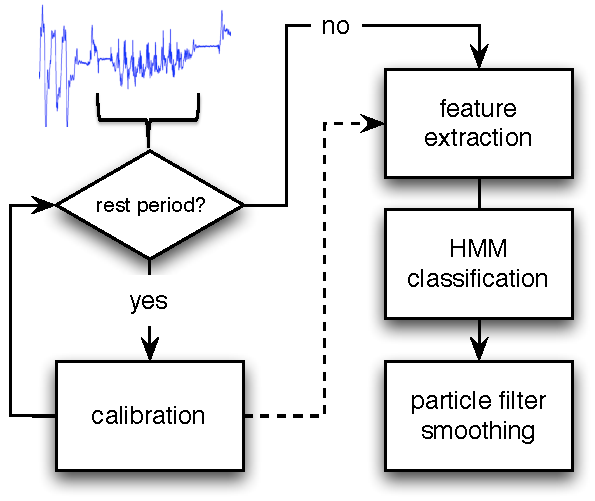
\includegraphics[width=3.5in]{hmm-overview}
\caption{Overview of the body placement recognition using HMMs}  
\label{fig:hmm-overview} 
\end{figure}

So far we just focused on placement detection while walking.
To overcome this activity limitation, we take the problem to the time
domain. For unconstrained motion data a naive sliding window approach won't work.
To do an unconstrained location recognition, it's
not enough to just look at a small snapshot in time. We need to shift our
attention to a statistical analysis over longer time intervals. 
We pick Hidden Markov Models (HMMs) as recognition algorithm, as they enable to 
encode the distinct motion patterns over time. They are  well explored in context
recognition research.  We train one HMM for each possible on-body
location. 

As the relative orientation of the accelerometer and gyroscope to the
body part are generally not known, we perform a constant orientation
calibration for one axis, described later in detail.

From a usage perspective, however, the HMMs have one major flaw. The HMM
classification for a specific body part will perform badly if it
receives uncharacteristic movement patterns from a specific body part.
Assuming that a change in body location is not too likely, the HMM is
limited by the time interval it takes into consideration.

A simple, naive procedure is to apply another majority decision
window~\cite{Kunze:2007p86}. This only helps to smooth over the
additional time interval. Therefore, we used a
particle filter for smoothing. It is able to remove small
disturbances and uncharacteristic patterns even over longer time periods.

In the following, we describe first the HMMs alone and second the
smoothing using a particle filter. Before discussing those
approaches, we will dive a little bit into the features used, as they
are essential for a successful recognition.


\subsubsection{Feature Calculation}
Feature extraction is fairly straight forward, we  use a one second sliding window
(0.5 sec overlapping) for the calculation.  We only perform feature extraction on segments
with enough activity.  If the variance of a segment on each axis tends
towards zero and the magnitude towards 9.81 m/s2, we assume this is
the gravity vector (see section~\ref{sec:orientationdetection} for
references and more details).  To account for sensor shifts and
displacements within a body part, we perform a constant orientation
calibration for one axis, as described by
Mizell~\cite{Mizell:2005p3885}. We perform feature extraction on this
vertical axis and the norm vector of the two vectors orthogonal to
gravity, if not indicated otherwise with the feature.  As an
additional feature we also use the length of the last calibration/rest period.

Our initial approach was to use a mixture of features that performed
well in the frame-by-frame case, presented
in Table~\ref{table:featuresWalking}.  Yet, those proofed to be suboptimal.
Table~\ref{hmmfeatures} lists the features we calculate on the
accelerometer and gyroscope data.


\begin{table}[ht]
\caption{Features used for the Hidden Markov Models}
\centering

\begin{tabular}{l l}
\toprule
Accelerometer & Gyroscope\\
\toprule
standard deviation and mean & PCA angle (Blanke et.al.~\cite{Blanke:2008p6128})\\
fft center of mass & frequency range power \\
duration of the last rest period & (below and above 2 Hz)\\\midrule
\multicolumn{2}{l}{\parbox[t]{\textwidth -2cm}{The sum of the norm of the differences in variance for the normalized axes $a_{1},a_{2},a_{3}$ divided by the variance of the vector norm: 
$\frac{1/2 \displaystyle\sum\limits_{i=1}^n \sum\limits_{j=1,j<i}^n\mid var(a_{i}) - var(a_{j})\mid}{var(norm)}$
}}\\
\bottomrule
\end{tabular}
\label{hmmfeatures}
\end{table}

\subsubsection{HMM Configuration}
The features are calculated as described above and a sequence of 5
min. feature segments are fed into continuous HMMs.  We use mixture
of 3-5 Gaussian distributions to estimate the HMM output
probabilities.  We train a separate HMM for each body placement.  Each
HMM in itself is fully connected. Depending on the placement
different numbers of hidden states are used: for the hand 5-6, torso 4, leg 5,
and for the head 4 hidden states. Training of each HMM is done by expectation maximization
using the Baum-Welch algorithm.  For evaluation, we feed the test
sequence in each placement specific HMM. There exists one HMM for each placement class. 
The HMM with the highest probability determines
the class assignment during the classification.  On top of the HMM only
classification, we use a majority decision window of size 10.

\subsubsection{HMMs with Particle Filter Smoothing}
The basic method for the HMM part stays the same. As we apply the
particle filtering we can reduce the sequence feed into the
individual HMMs to 45 sec. We input the 45 sec. sliding window HMM
classifications as observations into a particle filter. 
To our knowledge, particle filtering has not been applied
to this type of activity sensing problems.
Therefore, we will in the following go into more detail about
the method used.

\paragraph{Particle Filtering}

In case the majority window is too crude to filter out uncharacteristic
movements, we apply to this smoothing problem a  
partially observable dynamic model, a sequential monte carlo method, 
also called particle filter. The
theoretical part of this section is a summary from Andrieu, Doucet,
Thrun et. al. and Simon~(\cite{Andrieu:2003wb,Doucet:2001vx,Thrun:2001wc,Simon:2006p11115}). 
For a more detailed overview about filtering, especially more traditional
apporaches (Kalman etc.) please refer to Simon (\cite{Simon:2006p11115}).


Given we have the noisy classifications from the HMMs seen as
state observations  $y_{t_1},\ldots,y_{t_k}$ 
at times $t_1,\ldots,t_k$,  We want to estimate the hidden process states $x_{k}$.
We assume that the observations $y_k$ given $x_k$ is, if it is conditionally independent, distributed
according to the density function $g$, (see Equation~\ref{eq1}). 
We want to estimate the true body location state $x_{k}$ given the current and previous
"observations" $y_{k}$ (classifications of the HMMs).

\begin{equation}
    y_k|x_k \sim g(y_k|x_k)
    \label{eq1}
\end{equation}

To estimate the distribution $p(x_k|y_{1:k})$ the particle filter samples a reference density  $\pi(x_{t_k}|\{y_{t_i}\}^{k}_{i=1})$, sequentially with time $i$ from $1, \ldots, k$.
Particle filtering uses Bayesian estimation as the underlying principle
to make predictions about the current/future state given the past observations.
We use these predictions to smooth the results of HMM classifications.
Particle filtering adheres to the Markov assumption, every state depends only on the previous
state (Equation \ref{eq3}). 
Additionally, the measurements depend only on the current state (Equation \ref{eq4}).

\begin{equation}
p(x_k|x_{1:k-1}) = p(x_k | x_{k-1}) 
\label{eq3}
\end{equation}

\begin{equation}
    p(y_k|x_{1:k}) =p(y_k | x_{k}) 
\label{eq4}
\end{equation}

The relationship between measurements and system state is given in the Equations~\ref{pf:eq1}.
$u_k$ and $v_k$ are random noise with known distributions and 
$f$ and $h$ are known, arbitrary functions.
  
\begin{equation}
    x_k = f(x_{k-1}) + u_k \nonumber\\
\end{equation}
\begin{equation}
    y_k = h(x_k) + v_k 
    \label{pf:eq1}
\end{equation}

The prediction for the next state and update given a new measurement follows
the Bayes' Rule (see Equations~\ref{b:eq1} and \ref{b:eq2}).
The particle filter represents the posterior density, given in Formula~\ref{b:eq3},
as a set of $N$ random state vectors, called particles, denoted by $s_{1} ... s_{i}$ and
their associated weights $w_{1} ... w_{i}$.  We use a double index for the weights 
$(i,t)$, $i$ identifying the particle from $1 \ldots N$ and $t$ representing the time from $1 \ldots k$.
The posterior density is estimated over the weights.
The representation given in Equation ~\ref{pf:eq4} approaches the posterior density for very large numbers $N$.

\begin{equation}
p(x_k|y_{1:k-1}) = \int f(x_k | x_{k-1}) p(x_{k-1} | y_{1:k-1} ) \, dx_{k-1} 
\label{b:eq1}
\end{equation}

\begin{equation}
    p(x_k|y_{1:k}) = \frac{g(y_k|x_k) p(x_k|y_{1:k-1})}{ p(y_k|y_{1:k-1})}
\label{b:eq2}
\end{equation}

\begin{equation}
    where: p(y_k|y_{1:k-1}) = \int g(y_k|x_k) p(x_k|y_{1:k-1}) f(x_k|x_{k-1}) dx_k
\label{b:eq3}
\end{equation}


\begin{equation}
    \int f(x_k)p(x_k|y_{1:k})dx_k\approx\frac1N\sum_{i=1}^Nw_{i}f(x_{k,i}) 
    \label{pf:eq4}
\end{equation}


%\begin{equation}
%\int f(x_{t_k})| \{s_{t_j}\}^{k}_{j=1})dx_k\approx \frac{1}{N} \sum_{n=1}^N
%f(x^n_{t_k})\frac{p(x^n_{t_k}|\{s_{t_j}\}^{k}_{j=1})}{ \pi(x^n_{t_k}|\{s_{t_j}\}^{k}_{j=1})}
%\end{equation}

To reach a good estimate the particle filter performs iterative importance resampling steps given subsequently.
\begin{algorithmic}
\STATE 1. Draw $N$ particles from the proposed sampling distribution:\\$ s_t \sim \pi(x_{t}|s_{t-1},y_{t}) $
\FOR{$t=1$ to $k$}
\STATE 2. Compute and normalize the importance weight updates using the measurement $y_t$ according to: \\
${w}_{i,t} = w_{i,t-1} \frac{p(y_t|s_t) p(s_t|s_{t-1})} {\pi(s_t|s_{t-1},y_t)}$ 
\STATE 3. Re-sample, discarding any particle $s_i$ where the weight is smaller than a given threshold $w_{i,t} \leq w_{threshold}$.
\STATE 4. Predict $\hat{x}$ from $p_{x_t|x_{t-1}}(x|s_{1:t-1})$. 
\ENDFOR
\end{algorithmic}

The setup for the placement detection is as follows.
Each particle holds an estimate for the on-body placement class $c$ denoted by $c_1 ... c_j$ (e.g., leg, wrist).
The particles are initialized distributed equally with the placements of the data
set to evaluate.  The prediction model has a bias on not changing the
placement classification; the probability for keeping the location
class is set to steady 95 \%. 

To obtain a classification we use the
sum up over the weights of all particles $cs_{1,t} ...cs_{h,t}$ for a particular class.  As
seen in the evaluation section, reasonable results can be achieved
with around 60 particles.  


\section{Evaluation}
\label{onbodyeval}
Subsequently, we will look at the performance of the presented approaches
using some activity recognition data sets. We introduce first the different data sets and then go over the results.

\subsection{Data Sets}

All of the experimental setups for data sets use the XSens
XBus Master System\footnote{http://www.xsens.com} for recording motion
data. The XSens sensors combine a accelerometer, gyroscope and
magnetic field sensor. The opportunity data set contains in addition
bluetooth accelerometers. As indicated above, we use the acceleration and
rotation for our evaluation.
\begin{figure}[!t]
\centering
\begin{center}
    \subfloat[]{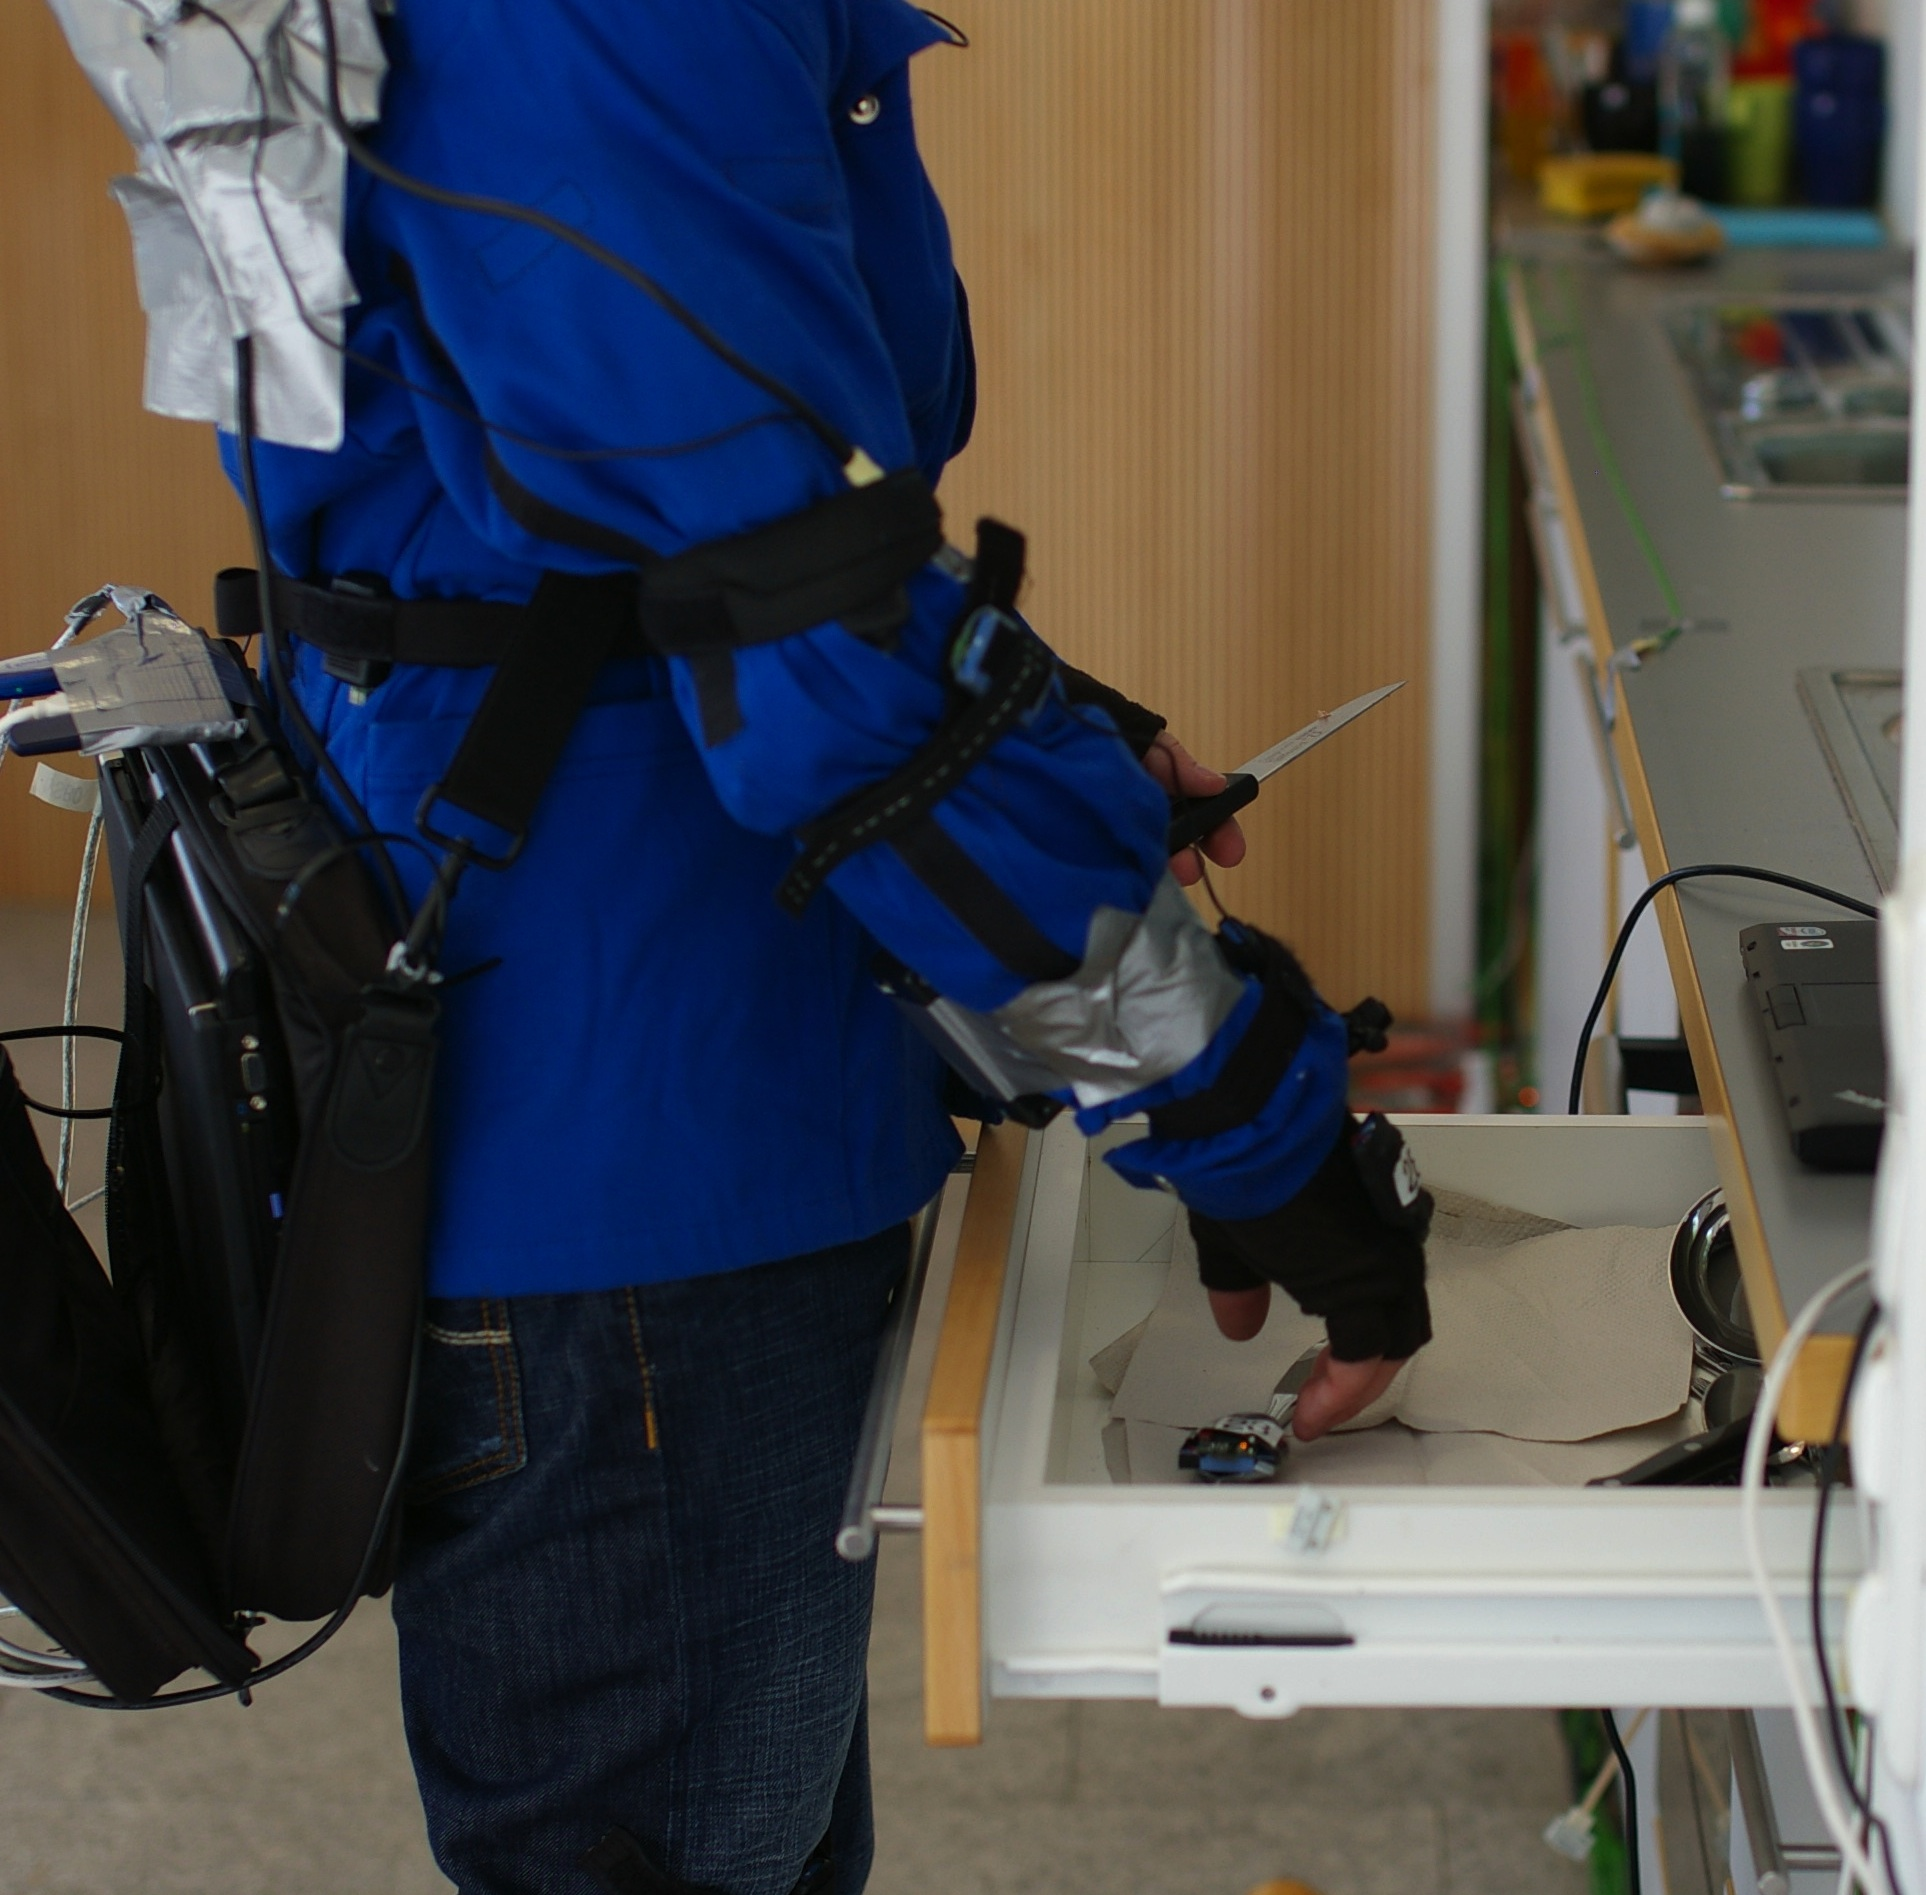
\includegraphics[height=1.3in]{exp1.jpg}
    	\label{fig:opp}}
     \subfloat[]{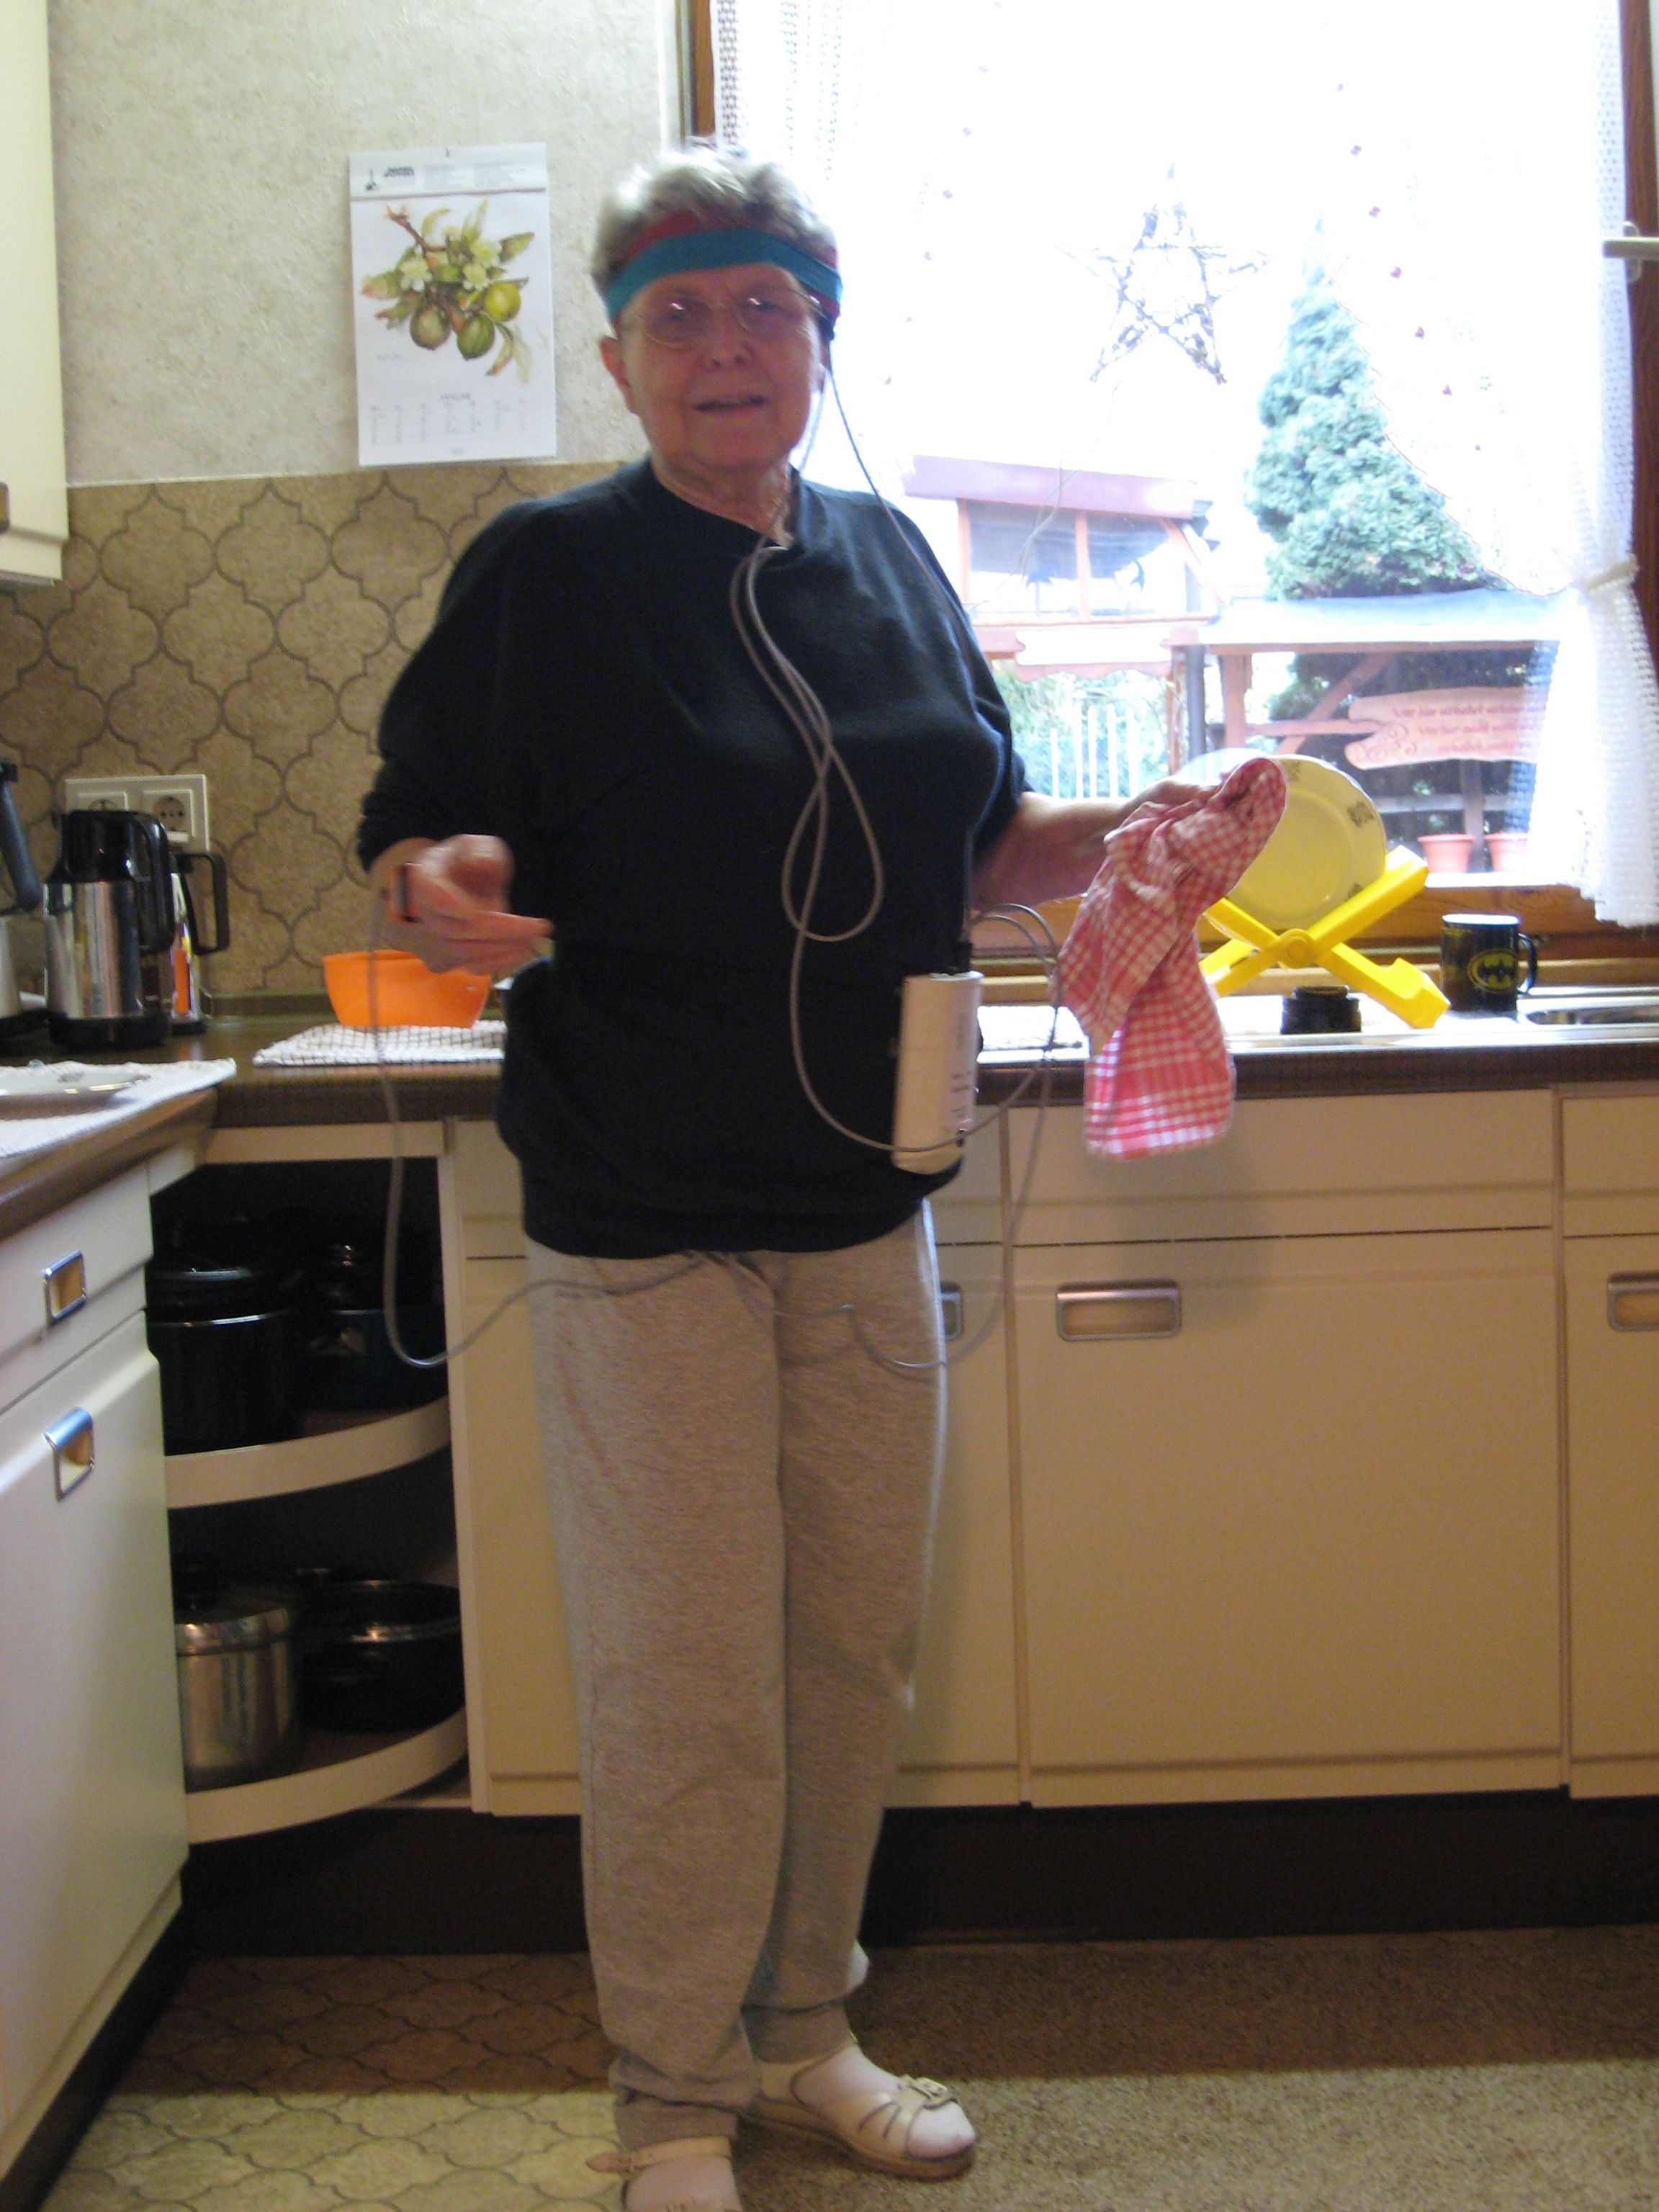
\includegraphics[height=1.3in]{exp5.jpg}
    	\label{fig:house}} \\   \end{center} 
     \subfloat[]{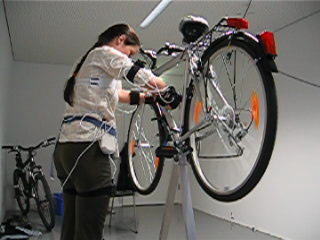
\includegraphics[height=1.12in]{exp4.png}
    	\label{fig:bicycle}}
     \subfloat[]{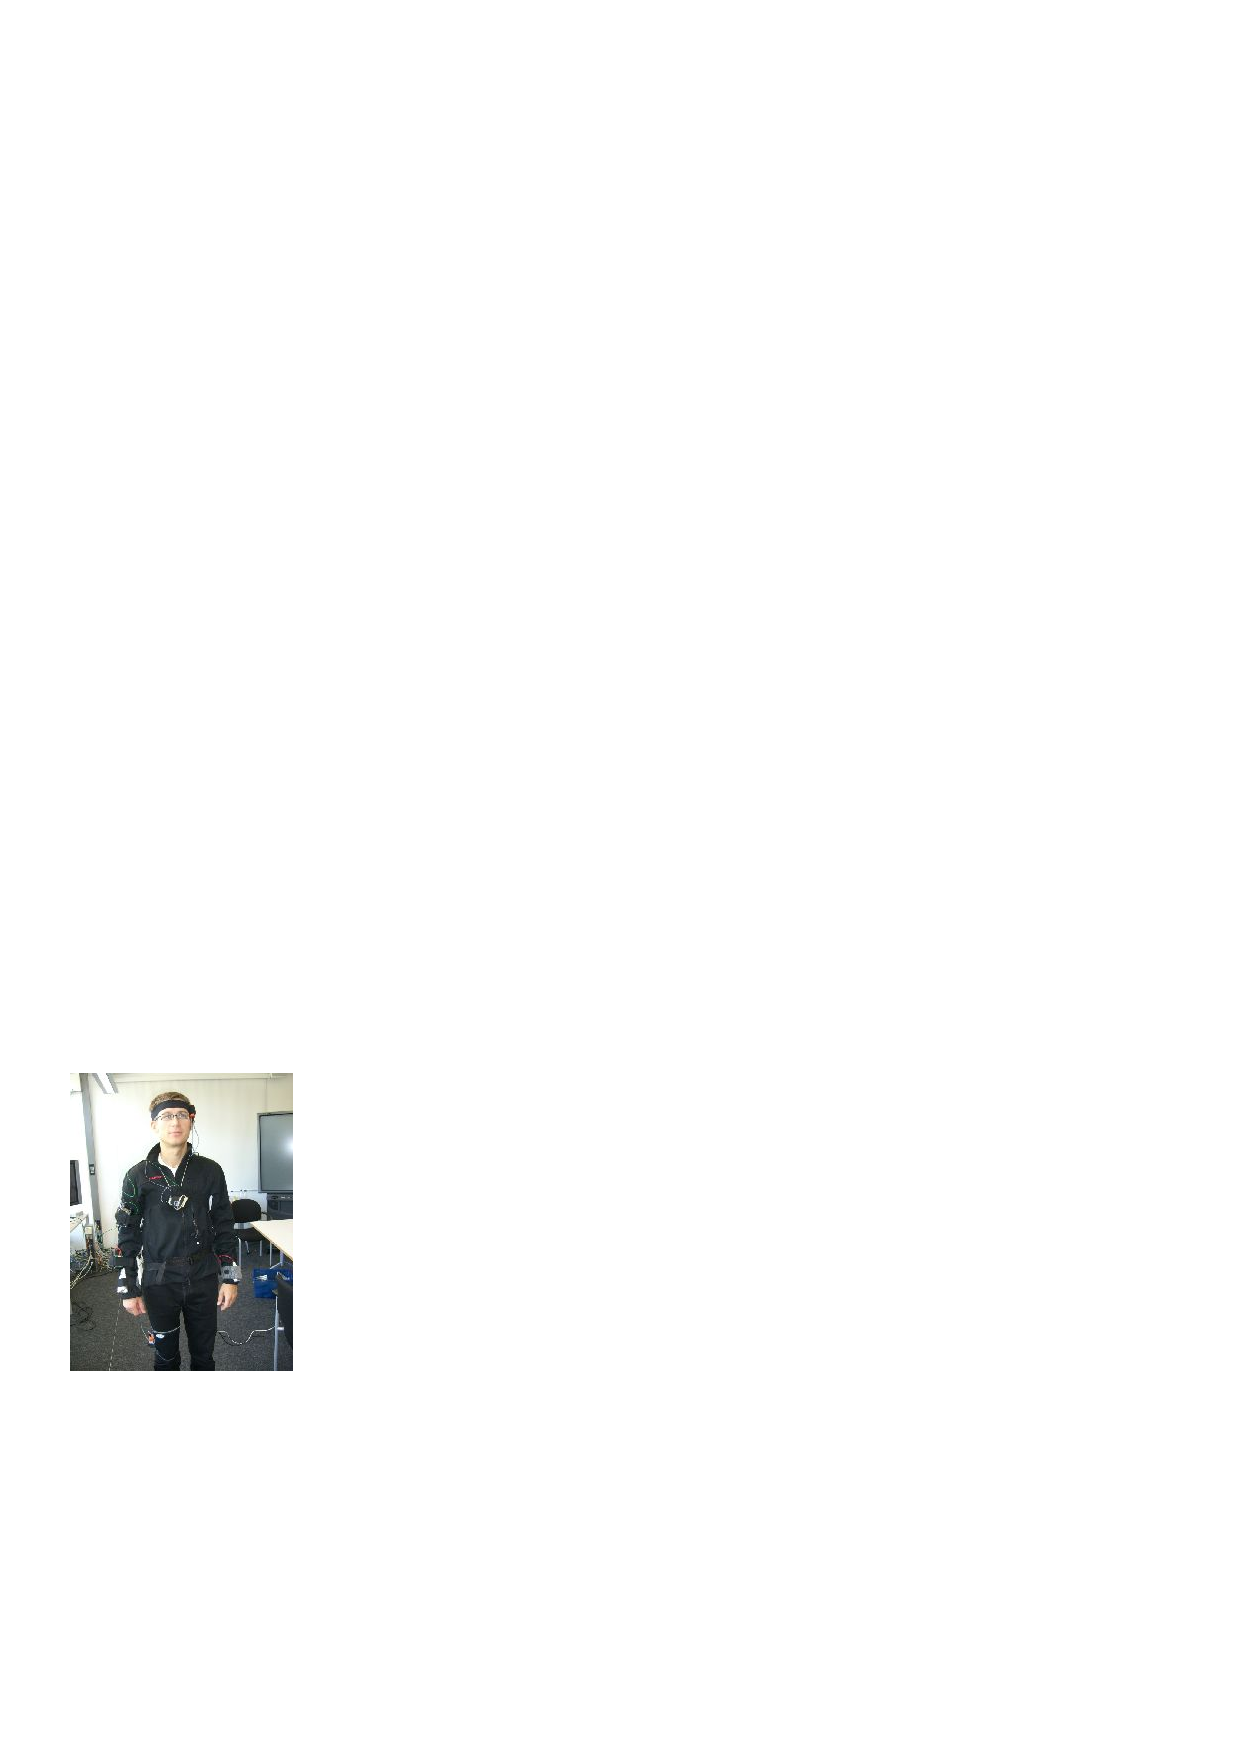
\includegraphics[height=1.12in]{exp3.pdf}
    	\label{fig:drink}}
     \caption[Pictures from the data collection]{Photos from the data collection of the data sets used. The Opportunity recordings in~\ref{fig:opp}, house work~\ref{fig:house}, 
     bicycle repair~\ref{fig:bicycle} and the Drink and work data set~\ref{fig:drink}.
       }
\label{fig:citytrace}
\end{figure}
Figure~\ref{fig:citytrace} shows pictures from the experimental setups
of the 4 different data sets used.

\emph{Office work} This data set contains 6 subjects. For each
subject, 3 experimental runs were recorded. Each run lasts between 12
and 15 minutes and consists of the following set of activities:
Working at a desk (writing emails, surfing, browsing through a book),
making coffee, giving a presentation, walking between the activities
(also including stairs). 4 Mtx Sensors are used. Sensor placements are
the wrist, right side of the head, left trouser pocket and left torso
pocket.

\emph{Opportunity} This data set was recorded as part of the
Opportunity EU Project. We use for our evaluation  7 users from  the data set with 5
runs per person. A usual run takes 15 to 25 minutes.
Thus, our evaluation set contains over 11 hours of
data. Activities are from everyday living and include "making a
sandwich", "pouring coffee", "eating" etc.  For the evaluation, we use the xbus jacket data (gyro
and acceleration) and the bluetooth accelerometer board sensor logs.
The xbus jacket locations are lower arm, upper arm, and back with a
sampling frequency of 30Hz.  The bluetooth accelerometer sensors are
attached to the back of the hand, wrist, upper arm, knee and hip with
a sampling frequency of 32Hz. The sensors were already used in
previous research \cite{Bachlin:2009p10850}. 

\emph{Drink and Work} This data set contains mostly sitting
activities, working on a computer and taking in food and drinks.  In
total 6 subjects are used in our evaluation; one experimental run is
around 30-40 min.  The Xsens motion sensors are attached at 5
locations, the upper back, right upper arm, right lower arm, head and
the upper leg, again with a 30 Hz sampling frequency.
Cheng et. al. describe more background information about the experimental setup~(\cite{Cheng:2010p10269}).

\emph{Bicycle Repair} This experimental setup contains repair
activities on a bike (attaching a tire, opening screws etc.) with 6
test subjects. The average recording is around 25 min., 2 experimental
runs for each subject. Again the xBus Master was used with sampling
rate at 50 Hz.  Only three placements are used: hand, lower and upper arm
(for details see~\cite{Stiefmeier:2006p10710}).

\emph{House Work} We conducted 3 experimental trials with 3 different
test subjects, each trial lasting over 1 hour.  We recorded real life
activities in four different scenarios: Kitchen work, washing and
ironing clothes, packing and office work. The data includes a wide
range of activities from drying dishes over folding shirts to making
coffee.  For the experiments, we used the xBus Master system.  These 
experiments are specifically recorded for the on-body placement
detection. Thus the placements are picked according to a study by
Ichikawa et. al.~\cite{Ichikawa:2005p6295} and are as follows: right
wrist, head, torso, front and back trousers pocket with 50 Hz sampling
frequency~\cite{Kunze:2007p86}.



\subsection{Walking Segments Method Results}
This method is applied to the Office Work and Opportunity data sets
only, as it requires long patches of walking by the users. 
Both data sets contain such long enough walking patches.

\paragraph{Placement Recognition on Segmented Data}
As already mentioned earlier, the location recognition is only done
during walking. Thus we begin our analysis by looking at the
performance of the placement recognition on  hand picked walking
segments. The results of the frame-by-frame recognition an all 90 segments
contained in the experimental data is shown in figure \ref{fig:comp}.
Using a majority decision on each segment leads to a 100\% correct
recognition (124 out of 124). The smallest segment is 1 minute long.

\begin{figure}[t]
\centering   
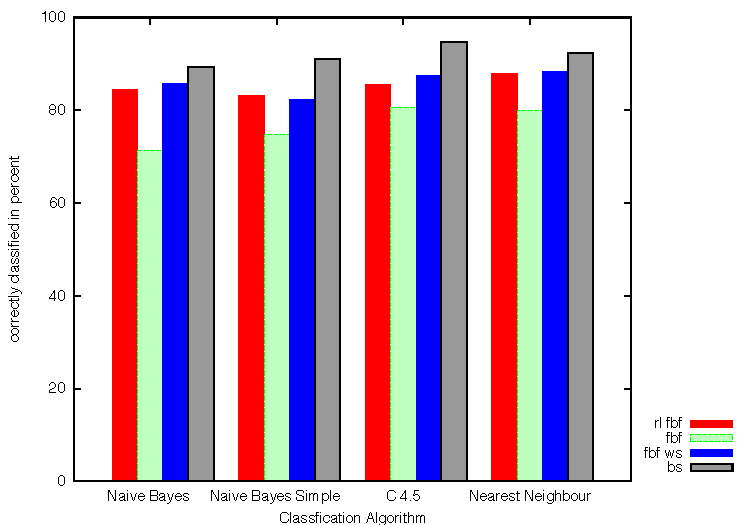
\includegraphics[scale=0.80]{comp.pdf}
\caption[Classification overview]{Overview over the different classification algorithms
and the varying approaches. The abbreviations have the following
meaning:   rl fbf =frame by frame using reference labeling
 fbf = for frame by frame location recognition using
frame by frame walking,  fbf ws = frame by frame location
recognition using smoothing over walking,  
bs = smoothing approach for
both location and walking.}
\label{fig:comp}
\end{figure}

\paragraph{Continuous Placement Recognition}
%\paragraph{Walking Recognition}
\label{walkingrec}
The first step towards placement recognition from a real life,
continuous  data stream is the detection of walking segments. 
As shown in Table \ref{table:walk} a frame-by-frame walking recognition
(walking vs. not walking) showed an accuracy 
between 69\% and 95\% (mean 82\%).
However, for our purpose the mere accuracy is not the main concern. 
Instead we are interested in minimizing the  number of false
positives, as the subsequent location recognition works correctly only
if applied to walking data. Here a mean of 18\%(over all experiments)
it is definitely too high.
\begin{figure}[t]
\centering   
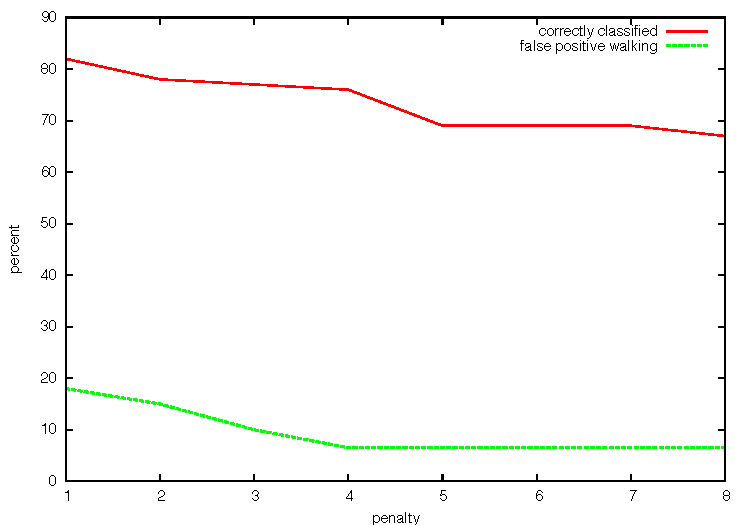
\includegraphics[scale=0.75]{fp.pdf}
\caption[Relation regarding false positives]{Relation between correctly classified and false positives for walking}
\label{fig:frame}
\end{figure}

\begin{figure}{h}
\centering   
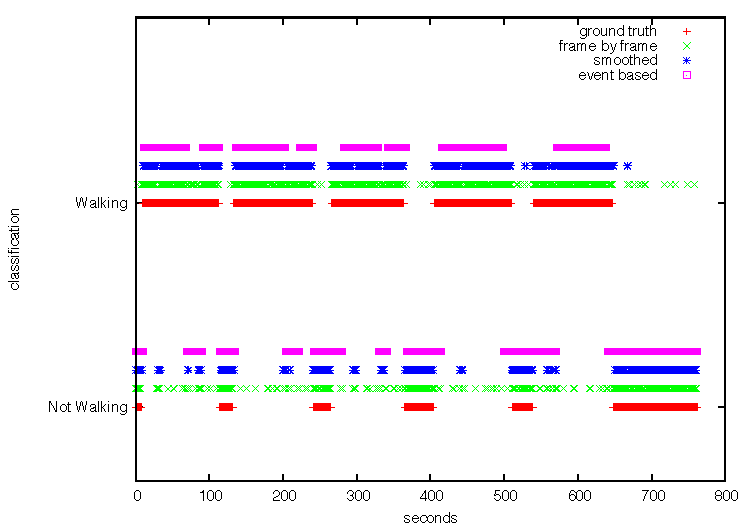
\includegraphics[scale=0.8]{wclass.pdf}
\caption[Sample for recognizing walking]{Sample set containing different approaches for recognizing the walking segments}
\label{fig:walk}
\end{figure}

As a consequence a false positive penalty has been added to the
classification algorithms. Tests (see Figure \ref{fig:frame}) have lead to
a minimal false positive 
rate considering a misclassification of 'Not Walking'  four times 
worse than a misclassification of 'Walking'. 
While 
the overall correct rates goes down to  between 61\% 
and 85\% (mean 76\%), the percentage of false positives for 'Walking'
is reduced to an average of 4\% (between 0.5\% and 7\%).\\
The best results for the walking recognition are provided by the C4.5 tree algorithm with a mean
of 82\%, the worst by the Naive Bayes Simple with 
a mean of 65\%.

\begin{table}[ht]
\caption[Frame by frame Overview]{Overview Classification for frame-by-frame walking recognition in percent,
user-dependent, per test subject(P1 to P6).}
\begin{tabularx}{\textwidth}{ l c c c c c c c}
\toprule                               
  & P1   & P2   &P3   & P4 & P5 & P6 & Mean\\ \hline
Plain  & & & & & & &\\
Correctly Classified &95 &69 &87 &78 &82 &85 &82.67\\
False Positives for Walking  &14 &8 &26 &10 &34 &18 &18.33\\\hline
With penalty  & & & & & & &\\
Correctly Classified            &83     &61     &78     &75     &79     &81     &76.17\\        
False Positives for Walking             &3      &5      &0.5    &8      &6      &6      &4.75\\\midrule
With penalty + jumping window  & & & & & & &\\
Correctly Classified             &93    &72     &89     &85     &78     &92     &84.83\\        
False Positives for Walking             &2      &3      &1      &2      &2      &3      &2.17\\ \bottomrule
\end{tabularx}
\label{table:walk}
\end{table}
In the next step, the effect of the jumping window smoothing we
described in previous research~(\cite{Kunze:2007p86}) was investigated. It showed an average
false positive rate of 2.17\%, with 84\% of the windows being correctly
recognized.

\paragraph{Walking Segments Location}
In the last walking recognition step the walking segment location was
applied to the smoothed frame by frame results. This has lead to 124
segments being located, none of which was located in a non-walking
section. As shown for an example data set in Figure \ref{fig:walk} the
only deviations from the ground truth was the splitting of single
segments and the fact that the detected segments were in general
shorter than the ground truth segments. In terms of suitability for
location recognition, however, this is not relevant.


\paragraph{Frame By Frame Placement Recognition}
\label{fbf}
With the walking segments detected the frame-by-frame placement recognition is
applied. The results are shown in Figure~\ref{fig:comp}. They are later improved using
the jumping window smoothing method which  leads to the results
shown in Figure~\ref{fig:comp} and Table~\ref{table:conf3}. 

\begin{table}[h]
\caption[Mean confusion matrix, frame by frame]{Mean of C4.5 over all data sets for pre-labeled frame-by-frame ( 89,81 \% correctly classified)}
\begin{center}
\begin{tabular}{|r c c c l|}\midrule
a	&b	&c	&d	&$\gets$ classified as\\\midrule
856	&2	&87	&5	&a = head\\
21	&804	&0	&12	&b = trousers\\
101	&32	&765	&4	&c = torso\\
0	&103	&5	&819	&d = wrist\\
\bottomrule
\end{tabular}
\label{table:conf}
\end{center}
\end{table}

\begin{table}[h]
\caption[Mean confusion matrix, frame by frame with segmentation]{Mean of C4.5 over all data sets for frame-by-frame using frame-by-frame walking recognition ( 80 \% correctly classified)}
\begin{center}
\begin{tabular}{|r c c c l|}\midrule
a	&b	&c	&d	& $\gets$ classified as\\\midrule
567	&4	&94	&4	&a = head\\
3	&431	&3	&178	&b = trousers\\
83	&32	&678	&10	&c = torso\\
12	&155	&24	&754	&d =wrist\\
\bottomrule
\end{tabular}
\label{table:conf2}
\end{center}
\end{table}

\begin{table}[h]
\caption[Mean confusion matrix with smoothing]{Mean of C4.5 over all data sets for both smoothed walking and location ( 94 \% correctly classified)}
\begin{center}
\begin{tabular}{|r r r r l|}\midrule
a       &b       &c      &d     & $\gets$ classified as\\\midrule
965     &2       &31     &2     &a = head\\
0       &847     &4      &49    &b = trousers\\
42      &0       &883    &1     &c= torso\\
17      &68      &10     &921   &d = wrist\\
\bottomrule
\end{tabular}
\label{table:conf3}
\end{center}
\end{table}

The confusion matrices depicted in Tables
~\ref{table:conf}~,\ref{table:conf2},~\ref{table:conf3} indicate that
the sensors attached to head and torso, as well as, trousers and
wrist are most often confused.  Especially, the confusion between Hand
and trousers is significant in size.  One possible reason is that the
movement pattern of Hand and Leg is similar while walking,
particularly if the test subjects swing with the arm.

\paragraph{Event Based Placement Recognition}
In a final step majority decision was performed in each segment leading
to an event based recognition. Just like in the manually segmented case
{\em the recognition rate was 100 \%}. 

We introduced a method that allows us to recognize where on the
user's body an acceleration sensor is located. The experimental
results presented above indicate that the method produces surprisingly
reliable results. The method has found all walking segments in each
experiment and has produced perfect event based recognition. Note that
for practical use such event based recognition and not the less
accurate frame by frame results are relevant.


\subsection{Hidden Markov Models Results}

\begin{table}[!t]
\centering
\caption{HMM Overview for several segment sizes}
\begin{tabular}{r r r r r r r}\toprule
Set / time & 30 sec. & 45 sec. & 1 min. & 3 min. & 4 min. & 5 min.\\
\midrule
Bicycle & 43 \% & 67 \% & -   & 83 \% & 83 \% & 84 \%\\
House & 32 \% & 65 \% & 68 \%  & 73 \% & 82 \% & 79 \%\\
Opp. (accel) & 20 \% & 59 \% & -  & 69 \% & 80 \% & 82 \%\\
Drink and Work & 15 \% & 61 \% & -  & - & 72 \% & 78 \%\\
\bottomrule
\end{tabular}
\label{overview}
\end{table}

Note that the walking segments methods has one severe limitation (despite just working on one particular activity).
It needs long walking segments to work. To overcome this issue,
we use Hidden Markov Models on unconstrained motion recordings.
As the walking segments are not crucial anymore, we can conduct
the following evaluation on all presented data sets.


\paragraph{Overall users}-- Table~\ref{overview} gives an overview about the HMM based classifications
on the different data sets for different segment duration. A segment
duration contains a vector of features shown in Table~\ref{hmmfeatures}
calculated over the 1 sec. sliding window. We use 33\% of the respective data set 
as training and 66 \% for evaluation. 

We get the best performance on the bicycle data set. However, as
there are only three on-body placements (lower arm, upper arm and hand),
the test subjects were all from a similar age group and since the whole
experimental setup was scripted, good results can be expected. 
The Opportunity accelerometer-only data performs surprisingly well,
even though the additional gyroscope information is missing. The Opportunity data set is
by far the largest, therefore the most representative data set. 
  The Drink and Work dataset performs worst of the data sets taking
5 min. before we reach an accuracy close to 80\%.  One possible reason
for this is that the test subjects are mostly stationary, sitting at a desk. 
Therefore, the movements can be quite uncharacteristic for the given body part.
The 45 sec. HMMs have an interesting threshold
of around 60\%, this is important as it proofs to be a decent start segment size 
for the particle filter later on. 


\begin{table}[!t]
\caption{Bicycle Repair with gyroscope and accelerometer 3 min. 83 \%}
\centering
\begin{tabular}{|r r r l|}\midrule
a &b &c &$\gets$ classified as\\\midrule
96.9 &1.2 &2.0 &a = hand\\
10.1 &69.7 &20.2 &b = lower arm\\
3.4 &11.4 &85.2 &c = upper arm\\
\bottomrule
\end{tabular}
\label{bicycle1}
\end{table}

\begin{table}[!t]
\caption[Bicycle Repair with accelerometer only]{Bicycle Repair with accelerometer only, 3 min. segment size, 76 \% accuracy}
\centering
\begin{tabular}{|r r r l|}\midrule
a &b &c &$\gets$ classified as\\\midrule
85.1 &12.9 &2.0 &a = hand\\
14.0 &66.7 &19.3 &b = lower arm\\
5.4 &13.0 &81.5 &c = upper arm\\
\bottomrule
\end{tabular}
\label{bicycle2}
\end{table}


\begin{table}[!t]
\caption{House Work  4 min. 82 \%}
\centering
\begin{tabular}{|r r r r r l|}\midrule
a &b &c &d &e &$\gets$ classified as\\\midrule
93.5 &4.9 &0.0 &1.6 &0.0 &a = head\\
0.0 &100.0 &0.0 &0.0 &0.0 &b = wrist\\
0.7 &0.0 &83.5 &15.8 &0.0 &c = torso\\
10.4 &1.4 &2.1 &81.9 &4.2 &d = back pocket\\
1.4 &0.3 &6.1 &24.2 &68.0 &e = front pocket\\
\bottomrule
\end{tabular}
\end{table}


\begin{table}[!t]
\caption{Opportunity XBus Jacket 2 min 90 \%.}
\centering
\begin{tabular}{|r r r l|}\midrule
a &b &c &$\gets$ classified as\\\midrule
90.5 &8.6 &0.9 &a = lower arm\\
10.0 &85.3 &4.7 &b = upper arm\\
0.0 &6.2 &93.8 &c = back\\
\bottomrule
\end{tabular}
\label{tab:opp}
\end{table}

\begin{table}[!t]
\centering
\caption[Opportunity accelerometer bluetooth nodes]{Opportunity accelerometer bluetooth nodes only 4 min 80 \%.}
\begin{tabular}{|r r r r r ||l|}\midrule
a &b &c &d &e &$\gets$ classified as\\\midrule
66.1 &9.3 &12.0 &10.1 &2.6 &a = hand\\
17.4 &76.2 &0.2 &0.5 &5.8 &b = wrist\\
8.4 &5.2 &81.6 &3.3 &1.5 &c = upper arm\\
9.5 &2.3 &0.8 &85.5 &1.9 &d = knee\\
1.1 &10.2 &0.1 &0.3 &88.3 &e = hip\\
\bottomrule
\end{tabular}
\end{table}


\begin{table}[!t]
\centering
\caption{Drink and Work 5 min. 78 \%.}
\begin{tabular}{|r r r r r l|}\midrule
a &b &c &d &e &$\gets$ classified as\\\midrule
73.1 &9.6 &15.2 &0.7 &1.4 &a = back\\
15.2 &70.2 &7.0 &5.8 &1.8 &b = head\\
7.2 &9.6 &76.0 &3.2 &4.0 &c = upper leg\\
0.0 &3.3 &0.8 &87.8 &8.1 &d = lower arm\\
3.9 &1.6 &0.8 &8.5 &85.3 &e = upper arm\\
\bottomrule
\end{tabular}
\label{drink}
\end{table}


The HMM results are summarized in the Tables~\ref{bicycle1}
to~\ref{drink} showing confusion matrices and overall accuracies.  


Comparing the Bicycle with the Opportunity xBus dataset (Tables~\ref{tab:opp} and~\ref{bicycle1}), 
it seems strange that the Bicycle scenario performs worse, as it also has only
3 classes. Even though the number of locations is equal, the locations
themselves are not. The xBus jacket locations (lower arm, upper arm,
back) are more diverse than the Bicycle repair ones (hand, lower and
upper arm). As the movements from the back can be easier distinguished
from the arm movements, the Opportunity dataset performs better.
Overall, the results in the confusion matrices are to be expected.
Body placements with similar movement patterns tend to be confused.

\begin{table}[!t]
\centering
\caption[HMM recognition rate]{HMM recognition rate (mean rate over several runs with different training sets) for user independent training, using 4 min segments.}
\begin{tabular}{r r r r r r}\toprule
Set / users for training & 1 & 2 & 3 & 4 & 5\\
\midrule
bicycle (6 users) & 27 \% & 42 \% & 45\%  & 50\% & 69 \%\\
house (3 users)  & 15 \% & 18 \% & - & - & -\\
opp. (accel, 7 users ) & 28 \% &36 \% & 40 \% & 48\% & 72 \%\\
drink and work (6 users) & 23 \% & 23 \% & 32 \% & 35\% & 52 \%\\
\bottomrule
\end{tabular}
\label{overview_ui}
\end{table}

\paragraph{User-independent} -- True user independence is only achieved
if we train on one (or multiple) users and evaluate on the rest, excluding
the users taken for training. Unfortunately, the HMM results in this 
case are not holding up to the good recognition rates seen before.
The results are summarized in Table~\ref{overview_ui}. 
The house work data set performs worst (less than mere chance).
It seems the user dependent characteristics dominate the classification,
therefore the recognition model is not generalizable over several users.
The data set contains also the most variability in user demographic.
For the opportunity and bicycle sets we see a clear increase for
the classification rates and the 5 user case is getting closer to 
the recognition performance over all users. 
This indicates that the approach introduced might work also
for the user-independent case. Yet, larger data sets are needed to
evaluate true user independence. It is out of scope for this thesis,
yet a promising research opportunity.

\subsection{HMMs and Particle Filter Results}

To show the usefulness of the particle filter on top of a HMM classification with a
smaller segment size (45 sec.), we perform 3 evaluations.
\begin{figure}[!t]
\centering
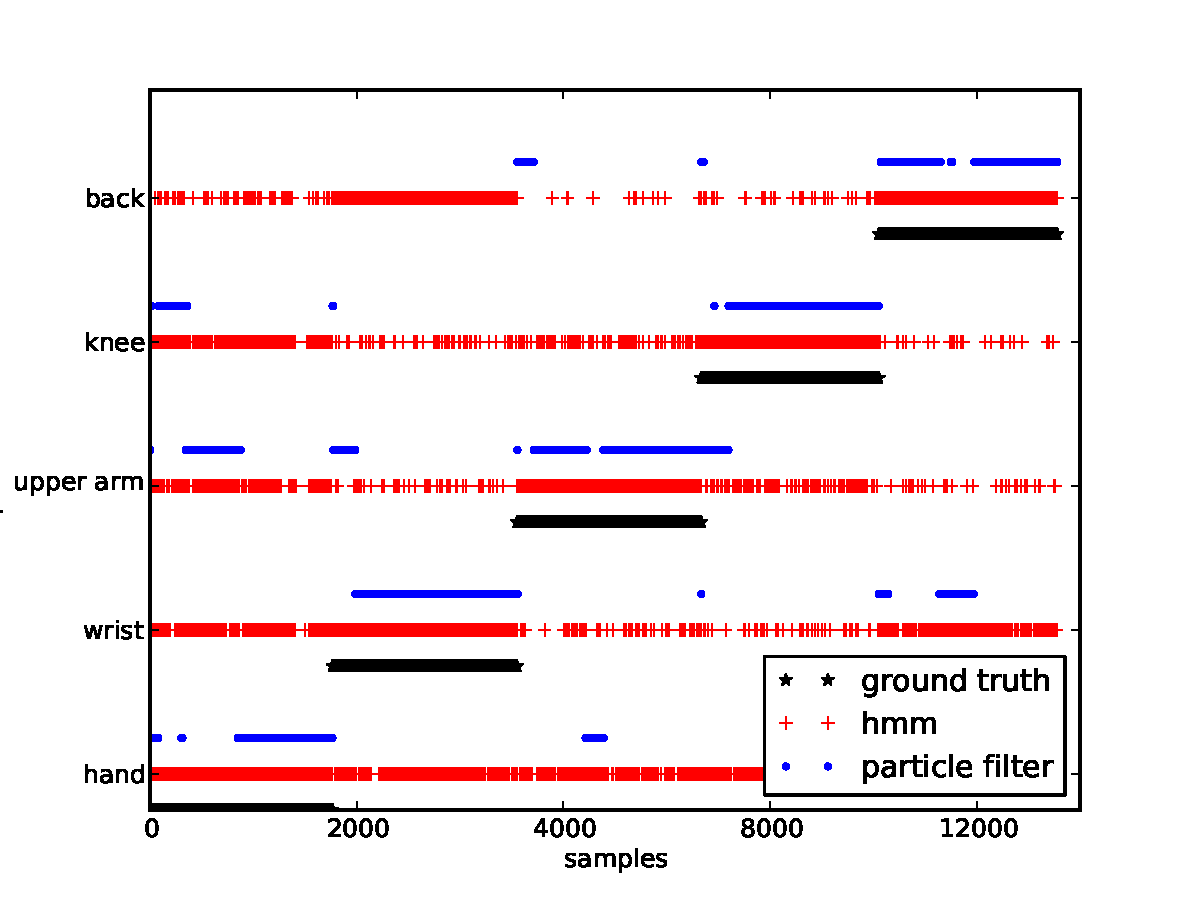
\includegraphics[width=2.5in]{scatter}
\caption[HMM Scatter Plot]{Scatter plot depicting the performance of the HMMs with and without particle filter smoothing. Here 20 min segments are taken
from the Opportunity Accelerometer only data, with 45 sec. HMM classification (around 59 \% correct). Achieving a 78 \% particle filter with 40 particles. }
\label{fig_scatter}
\end{figure}
The scatter plot in Figure~\ref{fig_scatter} clearly shows the smoothing effect
of the particle filter prediction.

\begin{figure}[!t]
\centering
\begin{center}
    \subfloat[]{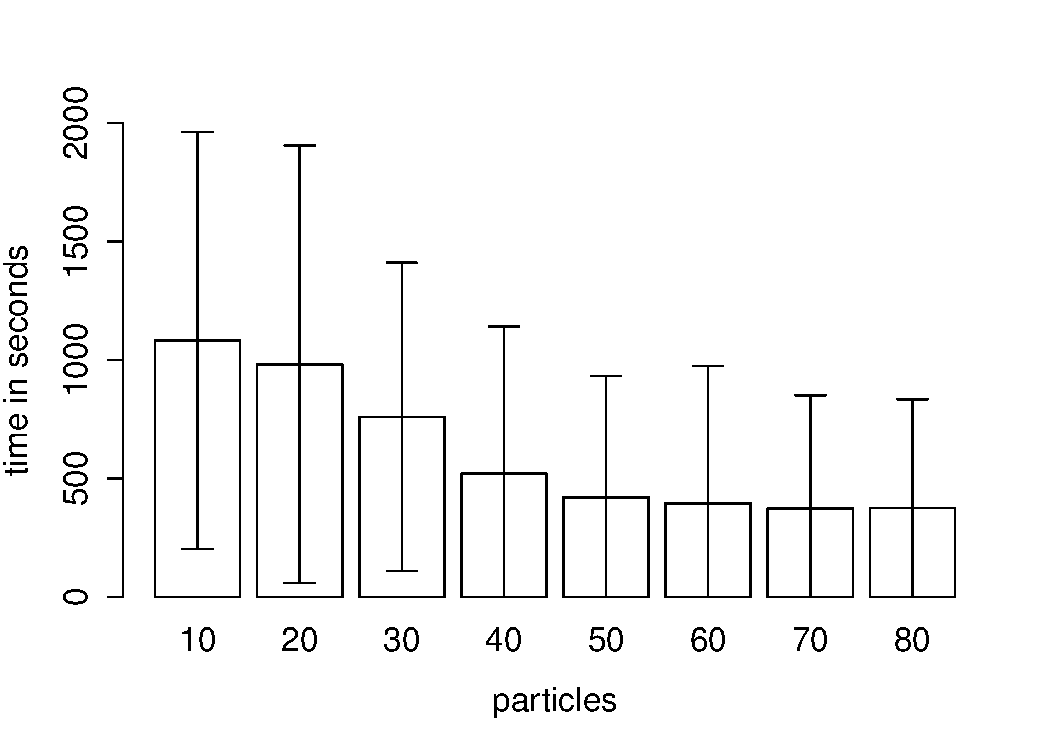
\includegraphics[height=1.7in]{opp3}
    	\label{fig_switchO}}
     \subfloat[]{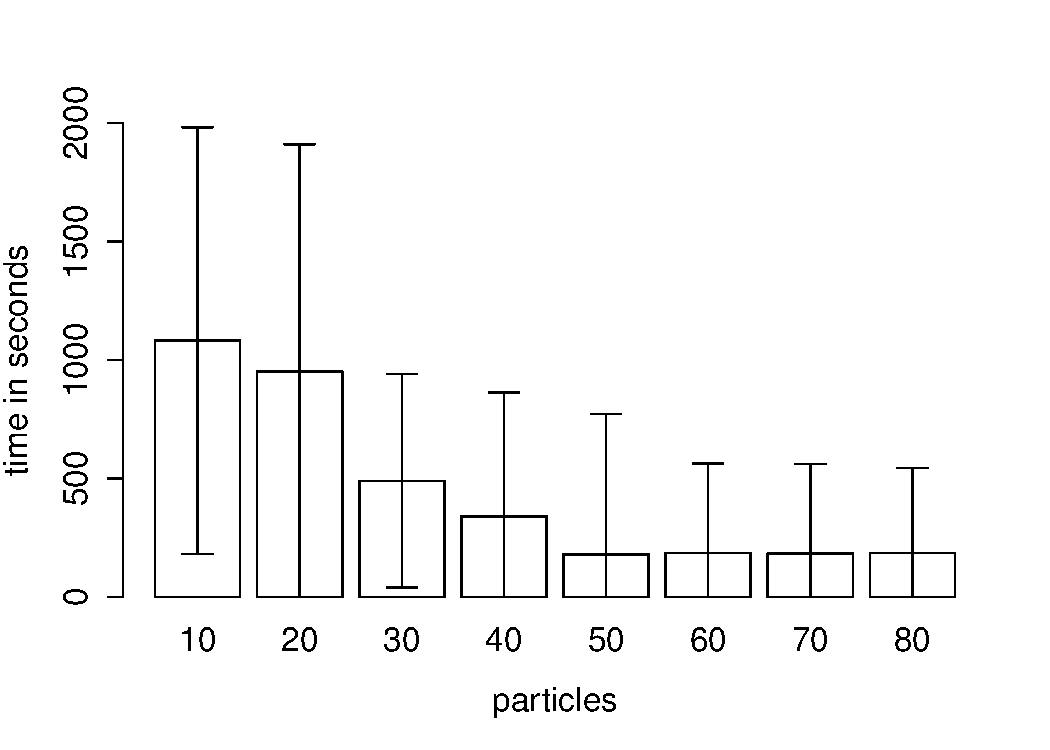
\includegraphics[height=1.7in]{bicycle3}
    	\label{fig_switchB}} \\   \end{center} 
     \subfloat[]{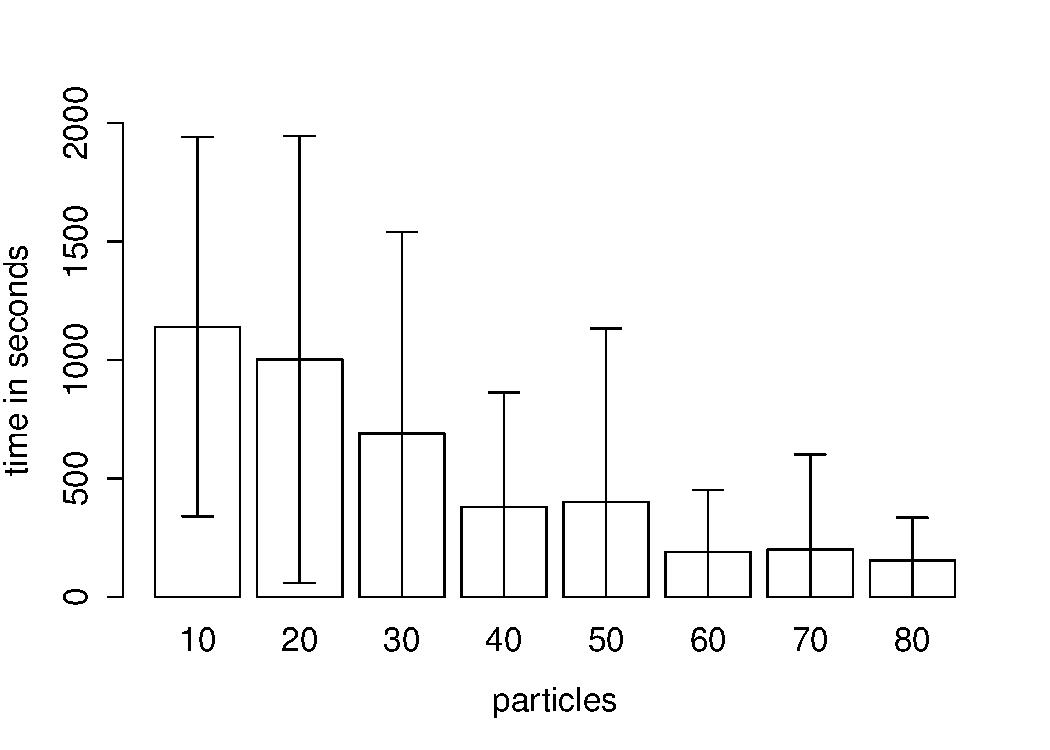
\includegraphics[height=1.7in]{drink3}
    	\label{fig_switchD}}
     \subfloat[]{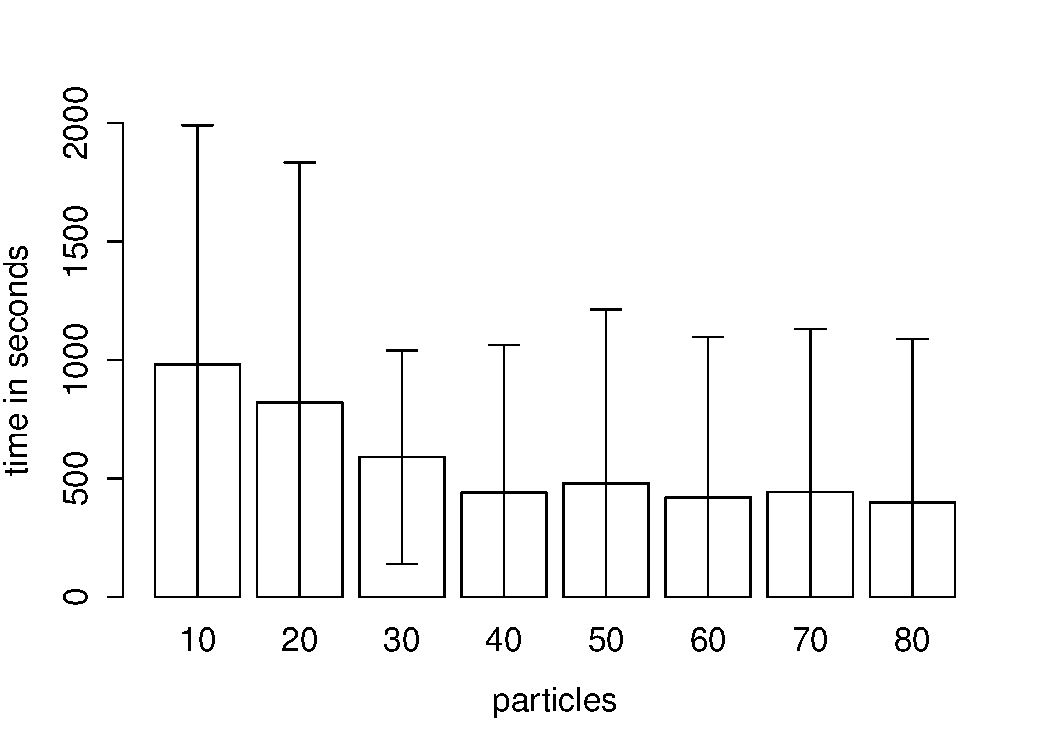
\includegraphics[height=1.7in]{house3}
    	\label{fig_switchH}}
     \caption[Particle filter mean and Standard deviation]{Mean and standard deviation of the switch time using 100 segments 
between 10 -20 min uniformly randomized for the opportunity (\ref{fig_switchO})
the bicycle repair(\ref{fig_switchB}), the drink and work (\ref{fig_switchD}) and
the house work data set(\ref{fig_switchH}).}
\label{fig:switch}
\end{figure}

\begin{figure}[!t]
\centering
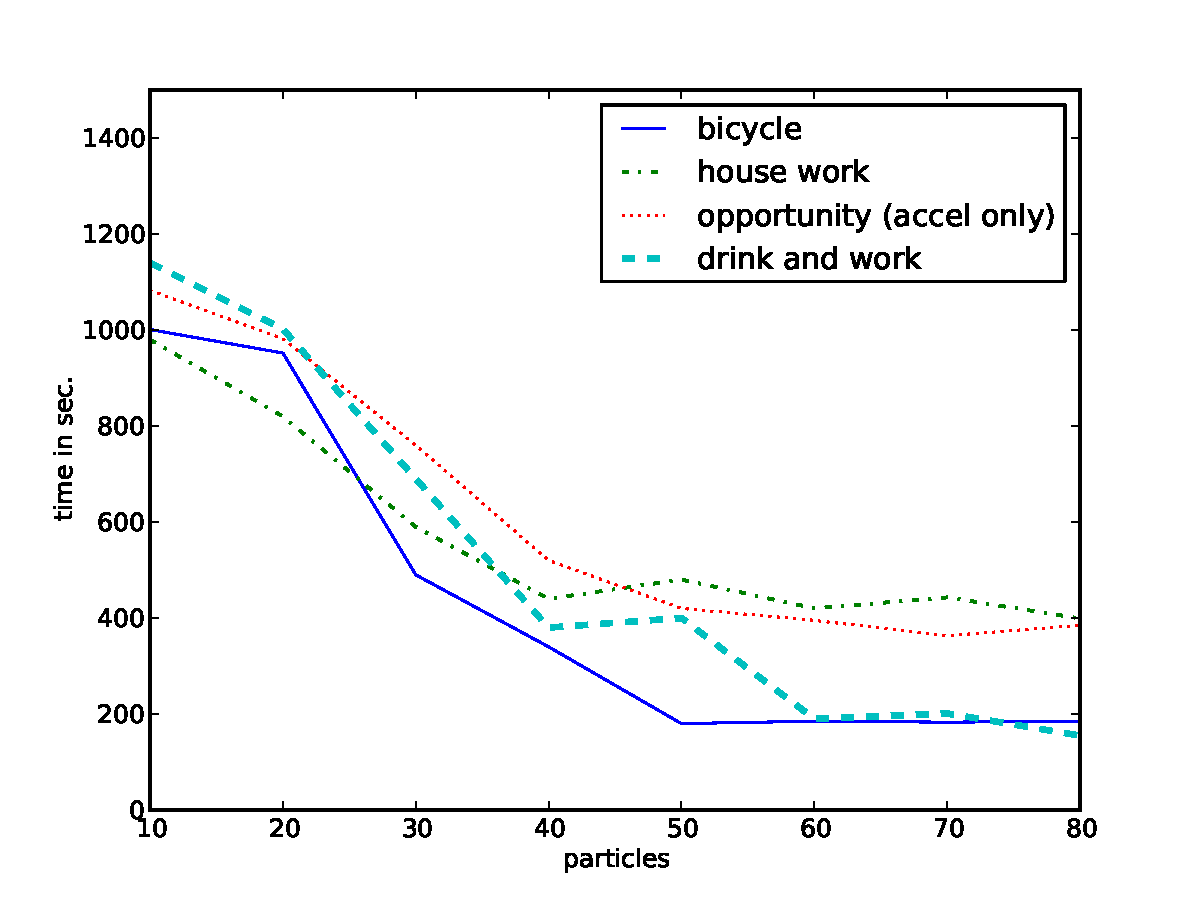
\includegraphics[width=2.5in]{allN}
\caption[Particle filter results, all datasets]{Mean and standard deviation of the switch time using 100 segments 
between 10 -20 min uniformly randomized for all data sets.}
\label{fig_allN}
\end{figure}


\begin{figure}[!t]
\centering
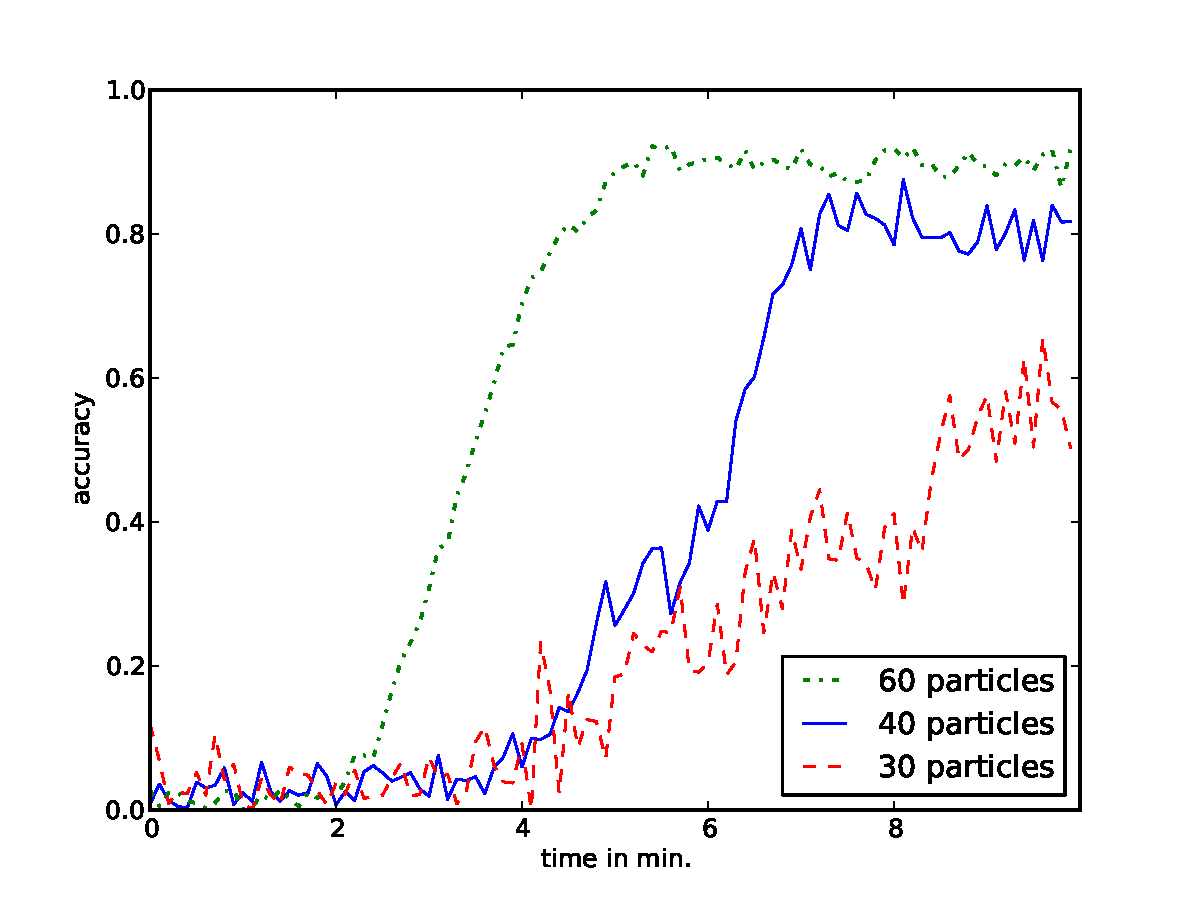
\includegraphics[width=2.5in]{all-opp}
\caption[Improvement using different particle numbers]{Classification improvement using different particle numbers for 100 x  10 min segments.}
\label{fig_particle}
\end{figure}


First of all, we determine the optimal amount of particles to use for
the filter.  We train our 45 sec. HMMs as
described in the Methods section.  We generate uniformly random 100
segments with 10 min. continuous accelerometer data from the test set
( there can be overlapping 10 min. pieces). On these 10 min pieces we
perform an evaluation for each time step and plot the average accuracy
and standard deviation for each data set, as seen in Figure~\ref{fig:switch}.
It is easier to compare the performance of the particle filter regarding
the different data sets in the summary Figure~\ref{fig_allN}.  
We can infer that a particle number of 60 seems a good pick for the data sets, as there is
no significant accuracy increase with 70 or 80 particles.

Another plot showing the performance of different particle sizes
is given in Figure~\ref{fig_particle} for the Opportunity data set.
The 60 particle case is more stable and smooth than the predictions with lower
particle numbers. It is important to note that the 1st sec. in the plot is the 45th sec. of the data, 
as this time is needed for the first HMM observation to appear.  

Second, we want to get the average timing for when the particle filter
supplies us with a stable reading and again a more general evaluation
on the particle size to use.  We use 100 time slices, uniformly random
between 10 and 20 minutes in size for this evaluation. House and
Opportunity accelerometer only data set require a long switch
time, around 6 min with 60 particles. Switch time is the time it takes before the majority of the particles show the
correct state. Whereas
the Bicycle repair and Drink and Work experiments are quicker with 3
and 4 min.  respectively. The drink and work data set also shows
significant improvements on higher particle numbers (towards 70 and 80
particles).  This holds true a bit for the opportunity accelerometer
only data set, however in this case only the standard deviation goes
down.

\begin{figure}[!t]
\centering
\includegraphics[width=2.5in]{summary}
\caption{100 x 10 min segments, 60 particles different data sets.}
\label{fig_summary}
\end{figure}

Third, to test our filter design, we uniformly randomly pick 100 x 10
min from the data sets (there can be duplicate parts), do feature
extraction and HMM classification and feed them into the particle
filter. Afterwards we evaluate how many percent of the 100 filtered
placements are detected correctly.  Figure~\ref{fig_summary} shows the
results for the different data sets.  As can be seen, the Office work
scenario performs best (using gyroscope and accelerometer), the Opportunity
data set is second (gyroscope and accelerometer).  The House Work starts off
quick (accel + gyro), yet does not achieve the average 90\% accuracy
and has the most variance from one filtered classification to the
other.



%\begin{figure}[!t]
%\centering
%\includegraphics[width=2.5in]{opportunity}
%\caption{Mean and standard deviation of the switch time using 100 segments between 10 -20 min uniformly randomized from the opportunity data.}
%\label{fig_switchO}
%\end{figure}

%\begin{figure}[!t]
%\centering
%\includegraphics[width=2.5in]{house}
%\caption{Mean and standard deviation of the switch time using 100 segments between 10 -20 min uniformly randomized from the house data.}
%\label{fig_switchH}
%\end{figure}

%\begin{figure}[!t]
%\centering
%\includegraphics[width=2.5in]{bicycle}
%\caption{Mean and standard deviation of the switch time using 100 segments between 10 -20 min uniformly randomized from the bicycle repair data.}
%\label{fig_switchB}
%\end{figure}

%\begin{figure}[!t]
%\centering
%\includegraphics[width=2.5in]{drink}
%\caption{Mean and standard deviation of the switch time using 100 segments 
%between 10 -20 min uniformly randomized from the drink and work data.}
%\label{fig_switchD}
%\end{figure}


We were a bit startled by the bad performance of the particle
filtering in the first 1-2 min. This is likely due to the particle
initialization; conceivably, it is possible to improve the start up
time by incorporating the first few HMM classifications with a
stronger bias or incorporate other knowledge. 
A logical continuation of this work is to design and conduct experiments
with realistic switch situations between device on-body placements, 
to get better priors and maybe to model the switch itself.


\section{Discussion}

We present several methods allowing us to derive the coarse device
placement solely based on rotation and acceleration signals from the
device. The methods work regardless of device orientation.  We
show an elaborate evaluation of these methods on already
published, large scale data sets with diverse activities from
bicycle repair to house work.  The recognition rate reaches up to 80\%
over 4 min. of unconstrained motion data for the worst scenario and
up to 90\% over a 2 min. interval for the best scenario.
\begin{figure}[!t]
\centering
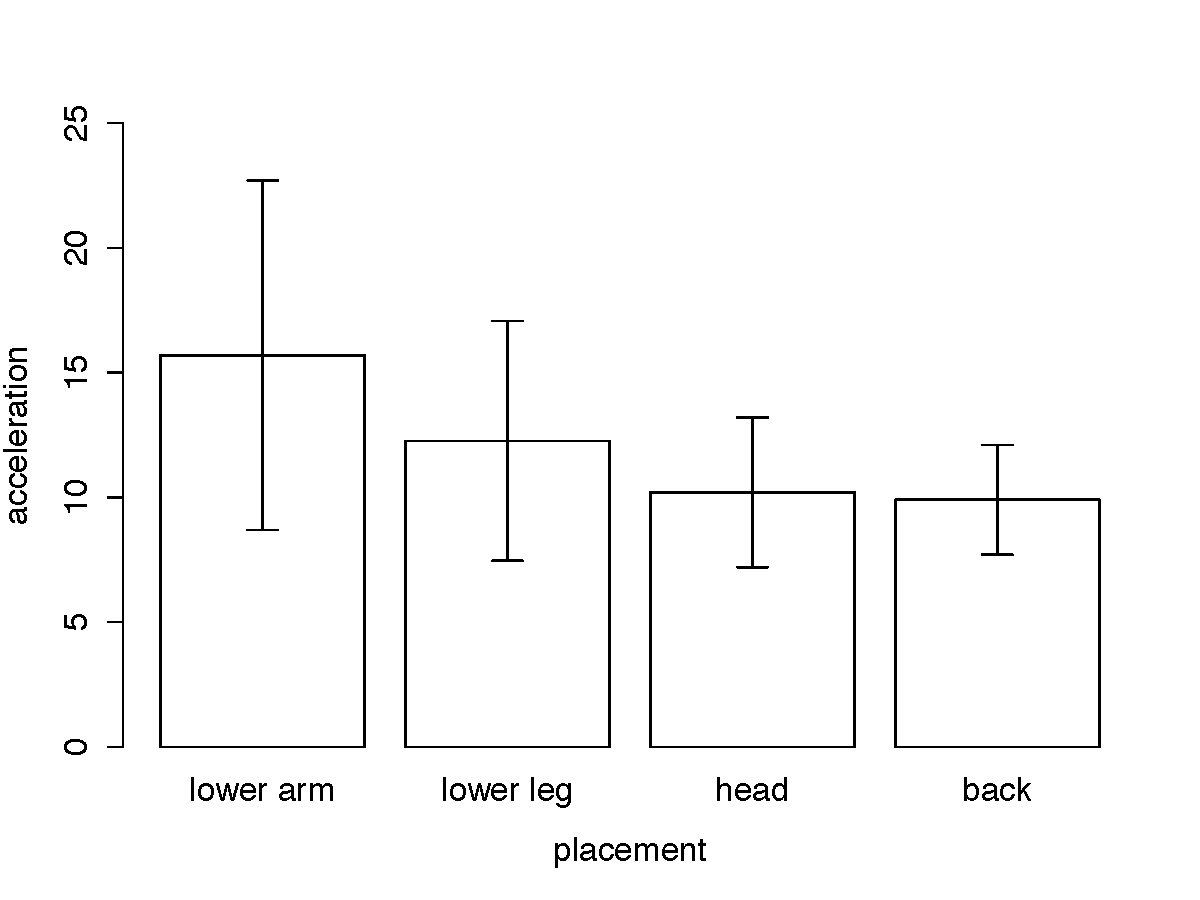
\includegraphics[width=2.5in]{placementComp}
\caption[Mean acceleration per location]{Mean and standard deviation of the acceleration (in $m/s^2$.
for different body locations over 2 users of the Drink and Work data set.}
\label{fig_loccomp}
\end{figure}
It seems the gyroscope features are very well
suited for distinguishing wrist and hand placements from the rest, as
one can also see from the confusion matrices in Tables~\ref{bicycle1}
and~\ref{bicycle2}.  Other than that, most missclassifications can be
easily explained, as they are from closely related placements (back
pocket and front pocket, hand and wrist etc.).  The Drink and Work
data set is worst in classification, this is due to the fact that the
person was stationary and sitting most of the time. The body parts
with less movement perform not that well (head and torso), as can
be seen from the confusion matrix in Table~\ref{drink}
and Figure~\ref{fig_loccomp}. Interesting here is that although it is worse in the HMM case, the
classification problems can be smoothed out with the particle filter.

The data set with the worst particle filter results, by far, is the
House work. Due to its variability of activities and the unscripted
nature of the recording, the accuracy highly depends on the used
training and test set. Also the diversity in test subject is highest with this experimental setup.  
The Opportunity
Bluetooth accelerometer data performs extremely well using the filter
smoothing, despite the fact that the data quality is considerably lower than that for the
Mtx Sensors and the additional gyroscope is missing. 
The impact isn't all that high, requiring roughly two minutes more run-time
for a stable particle filter performance compared to the Mtx sensor 
based inferences. This indicates that larger, more representative
data sets are essential.
 
There are several promising algorithmic alternatives and potential future work
regarding the on-body placement problem:

\begin{description}
\item{Conditional random fields} -- Recent activity recognition research 
applied an established inference framework from machine learning, conditional random fields (CRFs)
(\cite{Lafferty:2001:CRF:645530.655813,Vail:2007:CRF:1329125.1329409}).
They are more general than HMMs, in fact HMMs can also be expressed 
by CRFs. The major conceptional advantage of CRFs over HMMs is that they get rid of the 
independence assumption for the observations. As the observations
in the on-body placement method are all derived from acceleration and rotational 
velocity, this assumption is definitely violated, as with most HMM inferences in 
activity recognition research (\cite{790429,10.1109/ISWC.2005.22}). The CRF also don't need to rely on 
the Markov property. CRFs do not try to model the underlying process, conceptionally
they just predict the state according to the observations. There long  
observation interactions are feasible. Of course, one can imagine to also extend HMMs 
to overcome the Markov assumption, yet this is none-trivial and 
CRFs provide already a usable mathematical framework for it. Both, HMMs and CRFs are
similar in terms of complexity regarding the training and evaluation. 
Related work shows an improvement of the classification rate between 5-10 \%
using CRFs versus HMMs for similar activity recognition problems (\cite{Vail:2007:CRF:1329125.1329409}). 
Yet, if CRFs perform better than the HMM inference in the on-body placement case remains to be seen.
\item{Conformal Prediction} -- Conformal Prediction seems 
a good addition to the particle filter smoothing (\cite{Shafer:2008:TCP:1390681.1390693}). 
Its design targets online classification problems. 
Conformal Prediction gives solid confidence estimates for the next prediction of a system, even if the underlying
model of the system is not correct. In the on-body placement classification it can be used
to predict the confidence interval for the HMM classifications, the confidence in the prediction
can then in turn be used for the weights adjustment in the particle filter.
The method is quite novel in machine learning and not an established technique in the pervasive field.
Thus, it is also not tested on large scale activity sensing data sets.
Of course, Conformal Prediction can also be used to estimate the confidence of
the particle filter classifications. 
\item{Filtering adjustments} -- We use the particle filter to show the
best performance for the most general case, meaning we don't have any information
how often the user switches the device placement and where the user wears the
device regularly. Given a particular application domain and device type,
we can make certain assumptions (e.g. a mobile phone is often carried
 in the front pocket~\cite{Ichikawa:2005p6295}). 
Given these assumptions, depending on the application
scenario, the particle filter options can be adjusted 
accordingly (e.g. the prior distributions for a given location). 
This will lead to shorter switch times.
\end{description}

One other issue that future work can address is the
detection of location changes. The work described in this chapter
constitutes a first step towards the use of sensors integrated in
standard appliances and accessories carried by the user for complex
context recognition. It is also motivated by the relevance of device
location to infer the user's context.

%that happen when the user is not walking and short duration location
%changes occurring during walking (e.g. taking out a mobile phone
%events during walking).  Here, we see communication and cooperation
%between different devices as the key. Thus, for example, if all
%devices but the one located in a torso pocket detect walking then it
%must be assumed that something is happening to this device. Similar
%conclusions can be drawn if devices known to be in the trousers side
%pockets detect the user sitting and all but one devices report no or
%little motion while a single devices detects intensive movement. How
%such device cooperation can be used in real life situations and how
%reliable results it can produce is the subject of the next stage of
%our investigation.


 
\bibliographystyle{abbrv} \bibliography{onbody} % LocalWords: absorption
